% Options for packages loaded elsewhere
% Options for packages loaded elsewhere
\PassOptionsToPackage{unicode}{hyperref}
\PassOptionsToPackage{hyphens}{url}
\PassOptionsToPackage{dvipsnames,svgnames,x11names}{xcolor}
%
\documentclass[
  letterpaper,
  DIV=11,
  numbers=noendperiod]{scrartcl}
\usepackage{xcolor}
\usepackage{amsmath,amssymb}
\setcounter{secnumdepth}{-\maxdimen} % remove section numbering
\usepackage{iftex}
\ifPDFTeX
  \usepackage[T1]{fontenc}
  \usepackage[utf8]{inputenc}
  \usepackage{textcomp} % provide euro and other symbols
\else % if luatex or xetex
  \usepackage{unicode-math} % this also loads fontspec
  \defaultfontfeatures{Scale=MatchLowercase}
  \defaultfontfeatures[\rmfamily]{Ligatures=TeX,Scale=1}
\fi
\usepackage{lmodern}
\ifPDFTeX\else
  % xetex/luatex font selection
\fi
% Use upquote if available, for straight quotes in verbatim environments
\IfFileExists{upquote.sty}{\usepackage{upquote}}{}
\IfFileExists{microtype.sty}{% use microtype if available
  \usepackage[]{microtype}
  \UseMicrotypeSet[protrusion]{basicmath} % disable protrusion for tt fonts
}{}
\makeatletter
\@ifundefined{KOMAClassName}{% if non-KOMA class
  \IfFileExists{parskip.sty}{%
    \usepackage{parskip}
  }{% else
    \setlength{\parindent}{0pt}
    \setlength{\parskip}{6pt plus 2pt minus 1pt}}
}{% if KOMA class
  \KOMAoptions{parskip=half}}
\makeatother
% Make \paragraph and \subparagraph free-standing
\makeatletter
\ifx\paragraph\undefined\else
  \let\oldparagraph\paragraph
  \renewcommand{\paragraph}{
    \@ifstar
      \xxxParagraphStar
      \xxxParagraphNoStar
  }
  \newcommand{\xxxParagraphStar}[1]{\oldparagraph*{#1}\mbox{}}
  \newcommand{\xxxParagraphNoStar}[1]{\oldparagraph{#1}\mbox{}}
\fi
\ifx\subparagraph\undefined\else
  \let\oldsubparagraph\subparagraph
  \renewcommand{\subparagraph}{
    \@ifstar
      \xxxSubParagraphStar
      \xxxSubParagraphNoStar
  }
  \newcommand{\xxxSubParagraphStar}[1]{\oldsubparagraph*{#1}\mbox{}}
  \newcommand{\xxxSubParagraphNoStar}[1]{\oldsubparagraph{#1}\mbox{}}
\fi
\makeatother


\usepackage{longtable,booktabs,array}
\newcounter{none} % for unnumbered tables
\usepackage{calc} % for calculating minipage widths
% Correct order of tables after \paragraph or \subparagraph
\usepackage{etoolbox}
\makeatletter
\patchcmd\longtable{\par}{\if@noskipsec\mbox{}\fi\par}{}{}
\makeatother
% Allow footnotes in longtable head/foot
\IfFileExists{footnotehyper.sty}{\usepackage{footnotehyper}}{\usepackage{footnote}}
\makesavenoteenv{longtable}
\usepackage{graphicx}
\makeatletter
\newsavebox\pandoc@box
\newcommand*\pandocbounded[1]{% scales image to fit in text height/width
  \sbox\pandoc@box{#1}%
  \Gscale@div\@tempa{\textheight}{\dimexpr\ht\pandoc@box+\dp\pandoc@box\relax}%
  \Gscale@div\@tempb{\linewidth}{\wd\pandoc@box}%
  \ifdim\@tempb\p@<\@tempa\p@\let\@tempa\@tempb\fi% select the smaller of both
  \ifdim\@tempa\p@<\p@\scalebox{\@tempa}{\usebox\pandoc@box}%
  \else\usebox{\pandoc@box}%
  \fi%
}
% Set default figure placement to htbp
\def\fps@figure{htbp}
\makeatother


% definitions for citeproc citations
\NewDocumentCommand\citeproctext{}{}
\NewDocumentCommand\citeproc{mm}{%
  \begingroup\def\citeproctext{#2}\cite{#1}\endgroup}
\makeatletter
 % allow citations to break across lines
 \let\@cite@ofmt\@firstofone
 % avoid brackets around text for \cite:
 \def\@biblabel#1{}
 \def\@cite#1#2{{#1\if@tempswa , #2\fi}}
\makeatother
\newlength{\cslhangindent}
\setlength{\cslhangindent}{1.5em}
\newlength{\csllabelwidth}
\setlength{\csllabelwidth}{3em}
\newenvironment{CSLReferences}[2] % #1 hanging-indent, #2 entry-spacing
 {\begin{list}{}{%
  \setlength{\itemindent}{0pt}
  \setlength{\leftmargin}{0pt}
  \setlength{\parsep}{0pt}
  % turn on hanging indent if param 1 is 1
  \ifodd #1
   \setlength{\leftmargin}{\cslhangindent}
   \setlength{\itemindent}{-1\cslhangindent}
  \fi
  % set entry spacing
  \setlength{\itemsep}{#2\baselineskip}}}
 {\end{list}}
\usepackage{calc}
\newcommand{\CSLBlock}[1]{\hfill\break\parbox[t]{\linewidth}{\strut\ignorespaces#1\strut}}
\newcommand{\CSLLeftMargin}[1]{\parbox[t]{\csllabelwidth}{\strut#1\strut}}
\newcommand{\CSLRightInline}[1]{\parbox[t]{\linewidth - \csllabelwidth}{\strut#1\strut}}
\newcommand{\CSLIndent}[1]{\hspace{\cslhangindent}#1}



\setlength{\emergencystretch}{3em} % prevent overfull lines

\providecommand{\tightlist}{%
  \setlength{\itemsep}{0pt}\setlength{\parskip}{0pt}}



 


\KOMAoption{captions}{tableheading}
\makeatletter
\@ifpackageloaded{caption}{}{\usepackage{caption}}
\AtBeginDocument{%
\ifdefined\contentsname
  \renewcommand*\contentsname{Table of contents}
\else
  \newcommand\contentsname{Table of contents}
\fi
\ifdefined\listfigurename
  \renewcommand*\listfigurename{List of Figures}
\else
  \newcommand\listfigurename{List of Figures}
\fi
\ifdefined\listtablename
  \renewcommand*\listtablename{List of Tables}
\else
  \newcommand\listtablename{List of Tables}
\fi
\ifdefined\figurename
  \renewcommand*\figurename{Figure}
\else
  \newcommand\figurename{Figure}
\fi
\ifdefined\tablename
  \renewcommand*\tablename{Table}
\else
  \newcommand\tablename{Table}
\fi
}
\@ifpackageloaded{float}{}{\usepackage{float}}
\floatstyle{ruled}
\@ifundefined{c@chapter}{\newfloat{codelisting}{h}{lop}}{\newfloat{codelisting}{h}{lop}[chapter]}
\floatname{codelisting}{Listing}
\newcommand*\listoflistings{\listof{codelisting}{List of Listings}}
\makeatother
\makeatletter
\makeatother
\makeatletter
\@ifpackageloaded{caption}{}{\usepackage{caption}}
\@ifpackageloaded{subcaption}{}{\usepackage{subcaption}}
\makeatother
\makeatletter
\newcommand{\criticmarkupadd}[1]{#1}
\newcommand{\criticmarkuprm}[1]{}
\newcommand{\criticmarkupmark}[1]{#1}
\newcommand{\criticmarkupcomm}[1]{}
\makeatother
\usepackage{bookmark}
\IfFileExists{xurl.sty}{\usepackage{xurl}}{} % add URL line breaks if available
\urlstyle{same}
\hypersetup{
  pdftitle={Local Roots Within a National Political Divide: Evidence from a Split-Ballot Candidate Conjoint in Poland},
  pdfkeywords={friends-and-neighbors voting, local
candidates, government--opposition alignment, conjoint
experiment, Poland},
  colorlinks=true,
  linkcolor={blue},
  filecolor={Maroon},
  citecolor={Blue},
  urlcolor={Blue},
  pdfcreator={LaTeX via pandoc}}


\title{Local Roots Within a National Political Divide: Evidence from a
Split-Ballot Candidate Conjoint in Poland}
\author{}
\date{2026-09-09}
\begin{document}
\maketitle
\begin{abstract}
Territorial and partisan cues can both shape candidate evaluation, but
their relative weight across political alignments and offices remains
unclear. We examine these cues with a candidate conjoint embedded in the
2024 Polish Local Election Study. In a split-ballot design, 2,207
respondents evaluated four candidate pairs for member of parliament,
municipal councillor, or mayor and selected the profile better suited
for office. Residence in the municipality for a few years increased the
probability of selection by 13.4 percentage points relative to a
nonresident (parachute) profile, and lifelong residence increased it by
18.6 points. This gradient appeared in every office; neither the omnibus
interaction nor nine pairwise comparisons detected office differences.
Local roots and political alignment both mattered. Among clearly
positioned cases, profiles whose government stance matched the
respondent's gained 27.9--33.2 points over mismatched profiles. Even an
aligned outsider was 13.7 points more likely to be selected than a
non-aligned lifelong resident. The interaction between local roots and
political alignment varied across weighting and alternative alignment
cutoffs, so we treat it as exploratory. Local roots increase support
across political alignments, but they do not offset political mismatch.
\end{abstract}


\section{Introduction}\label{introduction}

\criticmarkuprm{Local roots need not
insulate}\criticmarkupadd{Territorial and partisan cues can coexist in}
candidate \criticmarkuprm{evaluation from national politics. In
polarized systems, voters may reward municipal embeddedness while still
ranking candidates through the national political divide. The central
question is therefore not simply whether candidates benefit near home,
but how local roots operate when national political alignment is
visible.}\criticmarkupadd{evaluation.} Friends-and-neighbors voting
(FNV) \criticmarkuprm{is a recurring pattern in electoral geography:
candidates receive}\criticmarkupadd{describes} disproportionate support
\criticmarkupadd{for candidates }where they live, were born, or
otherwise have a local connection (Key 1949; Lewis-Beck and Rice 1983;
Rice and Macht 1987; Gimpel et al. 2008). \criticmarkuprm{At the
national level, candidate--voter distance and candidate localness
predict vote choice}\criticmarkupadd{Local advantages appear} in
\criticmarkuprm{national}\criticmarkupadd{US state-legislative contests
(Hunt and Rouse 2023), parliamentary} elections (Arzheimer and Evans
2012; Górecki and Marsh 2012; Evans et al. 2017; Hunt 2022), intraparty
competition ({Put et al.} 2020), and \criticmarkuprm{evaluations of
party leaders (Put 2021). At the subnational level, local advantages
appear in a Polish open-list council election and Polish rural mayoral
elections (Czapiewski and Woźniak 2021; Górecki et al. 2022), German
local executive elections (Zissel 2026), and US state-legislative
contests (Hunt and Rouse 2023). These observational
associations}\criticmarkupadd{Polish and German local elections
(Czapiewski and Woźniak 2021; Górecki et al. 2022; Zissel 2026).
Observational estimates} combine \criticmarkuprm{several processes.
Local information declines with distance (Bowler et al. 1993), while
locally rooted candidates may canvass more, draw
on}\criticmarkupadd{information, canvassing,} personal networks,
\criticmarkuprm{enjoy greater }name recognition, \criticmarkuprm{or
mobilize nearby voters.}\criticmarkupadd{and mobilization.} Field
experiments \criticmarkuprm{confirm}\criticmarkupadd{show} that appeals
to \criticmarkuprm{shared geography}\criticmarkupadd{candidates' local
roots} can increase turnout (Panagopoulos et al. 2017; Panagopoulos and
Bailey 2020), but \criticmarkuprm{they do }not \criticmarkuprm{show
where place-based evaluation sits relative to a
national}\criticmarkupadd{how territorial cues compare or interact with}
political \criticmarkuprm{cue.}\criticmarkupadd{alignment.}

\criticmarkuprm{Survey and ballot-information}\criticmarkupadd{Candidate
conjoint} experiments \criticmarkuprm{show that residence affects
candidate evaluations when profiles provide comparable information
(Campbell and Cowley 2014; Harfst et al. 2023). Recent work has examined
expectations of local service, place identity, community embeddedness,
and localistic appeals (Campbell et al. 2019; Schulte-Cloos and Bauer
2023; Velimsky et al. 2024; Munis and Burke 2023; Nyholt 2024; Ornstein
et al. 2025). These studies do not support}\criticmarkupadd{can isolate
several signals within a common choice environment (Hainmueller et al.
2014; Schwarz and Coppock 2022). We contribute three comparisons in} one
\criticmarkuprm{universal mechanism, and several caution that residence
duration bundles multiple possible inferences. Localism is graded, yet
research often reduces it to a local--non-local distinction, and usually
studies that distinction apart from national political congruence.
Parties also field recognizable ``parachute'' candidates with no prior
connection to a constituency (Arter and Poyet 2024).
We}\criticmarkupadd{study. First, we} compare three
\criticmarkuprm{complete municipal-connection statements---lifelong
residence, residence for}\criticmarkupadd{degrees of municipal
connection rather than} a \criticmarkuprm{few
years,}\criticmarkupadd{binary local--non-local treatment. Second, we
hold the set of randomized profile attributes constant across MP,
mayoral,} and \criticmarkuprm{residence
elsewhere}\criticmarkupadd{councillor prompts. Third, we examine whether
the local-roots bonus varies} with \criticmarkuprm{declared local
knowledge---and locate their effects within the national
government--opposition divide.}\criticmarkupadd{respondent--candidate
political alignment in a polarized setting.}

\criticmarkuprm{Candidate conjoint experiments}\criticmarkupadd{Poland
combines a durable, affectively polarized government--opposition divide
(Tworzecki 2019) with electoral institutions that leave room for
candidate-level and territorial cues. Open-list elections encourage
personal-vote competition (Shugart et al. 2005), while independent lists
and mayors remain prominent in municipal politics (Gendźwiłł 2012).
Municipal elections} can \criticmarkuprm{compare several
candidate}\criticmarkupadd{also convey second-order} signals
\criticmarkuprm{within}\criticmarkupadd{from the parliamentary arena:
national governing parties often lose support, although comparative
evidence shows that this pattern is conditional (Gendźwiłł and Kjaer
2023). This combination makes Poland} a \criticmarkuprm{common choice
environment (Hainmueller et al. 2014; Schwarz and Coppock 2022).
Existing applications show that}\criticmarkupadd{useful setting for
comparing} local \criticmarkuprm{ties matter in candidate selection
among party elites (Berz and Jankowski 2022) and alongside party labels
among voters in a polarized US setting (Munis 2021). Our design connects
three comparisons in one argument. The graded treatment establishes
whether stronger municipal embeddedness increases support. The alignment
comparison tests whether national congruence can outweigh those local
roots. The split-ballot office comparison tests whether the local
advantage is confined to specifically local
offices.}\criticmarkupadd{roots with political alignment.}

We use a candidate conjoint embedded in the 2024 Polish Local Election
Study (PLES) (Gendzwill and Kroszka 2025). \criticmarkuprm{Poland
provides a demanding comparison because party competition is organized
around a durable, affectively polarized government--opposition divide
(Tworzecki 2019). }Respondents were randomly assigned to evaluate
candidates for MP, municipal councillor, or mayor.
\criticmarkuprm{Every}\criticmarkupadd{Each} condition used the same
\criticmarkupadd{set of }randomized attributes, including municipal
connection and attitude toward the current national
\criticmarkuprm{government. This national cue is not a party label, but
it locates profiles relative to the principal partisan divide and tests
whether that divide structures subnational candidate
evaluation.}\criticmarkupadd{government.}

\criticmarkuprm{The three comparisons support one claim: local roots
matter, but they operate within rather than outside the national
political divide. }Stronger municipal
\criticmarkuprm{embeddedness}\criticmarkupadd{connection} increases
\criticmarkupadd{the probability of }selection, and
\criticmarkuprm{this}\criticmarkupadd{the} gradient appears across all
three offices. \criticmarkuprm{Yet aligned}\criticmarkupadd{Local roots
and political alignment both matter. Among clearly positioned cases,}
profiles \criticmarkupadd{whose government stance matches the
respondent's }gain 27.9--33.2 percentage points over
\criticmarkuprm{non-aligned}\criticmarkupadd{mismatched} profiles. An
aligned \criticmarkuprm{profile with the outsider-with-local-knowledge
statement}\criticmarkupadd{outsider} even outperforms a non-aligned
\criticmarkuprm{profile with the lifelong-resident
statement}\criticmarkupadd{lifelong resident} by 13.7 points. The
primary model suggests a larger lifelong-residence bonus among aligned
pairs, but this interaction \criticmarkuprm{weakens under
alternative}\criticmarkupadd{varies across} weights and
\criticmarkuprm{attitude cutoffs.}\criticmarkupadd{alternative
definitions of political alignment. We therefore treat the interaction
as exploratory: local roots increase support in both groups, but they do
not offset political mismatch.}

\criticmarkuprm{The evidence establishes how respondents react to the
randomized statements, not why they value local candidates. Because the
outsider statement also declares local knowledge, the experiment
estimates complete statement contrasts rather than residence alone. It
likewise cannot identify campaign effort, personal acquaintance, or
network mechanisms.}

\section{Local Roots Within the National Political
Divide}\label{local-roots-within-the-national-political-divide}

\subsection{Graded municipal
embeddedness}\label{graded-municipal-embeddedness}

\criticmarkuprm{Voters use observable}\criticmarkupadd{Survey and
ballot-information experiments show that residence affects} candidate
\criticmarkuprm{traits}\criticmarkupadd{evaluations when profiles
provide comparable information (Campbell and Cowley 2014; Harfst et al.
2023). Other studies link the local-candidate advantage to expected
local service (Campbell et al. 2019), place identity (Schulte-Cloos and
Bauer 2023), and community embeddedness (Ornstein et al. 2025), while
finding that residence preferences are not reducible to one mechanism
(Nyholt 2024). These findings make both behavioral
localism---expectations about representation or service---and symbolic
localism---attachment to a candidate perceived} as
\criticmarkuprm{shortcuts when information is limited (Popkin 1991;
Lupia 1994; Lau and Redlawsk 2006), a pattern confirmed across recent
candidate-choice experiments (Schwarz and Coppock 2022). Municipal
connection may signal knowledge}\criticmarkupadd{part} of
\criticmarkuprm{local problems, shared interests, post-election
accessibility, accountability, or embeddedness in local networks. These
inferences need not be correct, and they do not require personal
acquaintance.}\criticmarkupadd{the community---plausible.}

\criticmarkuprm{Local connection is not binary.}\criticmarkupadd{Most
experiments nevertheless compare one local category with one non-local
category.} Local political experience and birthplace can have different
electoral implications (Tavits 2010), \criticmarkuprm{while place
identity can benefit hometown candidates even when they have little
prospect of winning (Schulte-Cloos and Bauer 2023). Lifelong residents,
newer residents, }and
\criticmarkuprm{outsiders}\criticmarkupadd{residence duration} may
\criticmarkuprm{therefore }convey different degrees or kinds of
proximity. \criticmarkuprm{Most experimental studies compare a local
candidate}\criticmarkupadd{Parties also field recognizable parachute
candidates} with \criticmarkuprm{a non-local candidate; the three-level
treatment tests whether voters distinguish positions within that broad
divide.}\criticmarkupadd{no prior constituency connection (Arter and
Poyet 2024). The first extension therefore treats municipal connection
as graded rather than binary.}

\criticmarkuprm{We expect both resident statements to outperform the
outsider statement and lifelong residence to produce the largest
place-based bonus. The outsider's declaration of local knowledge
resembles a common defense of parachute candidacy: connection is
asserted despite non-residence. This wording makes the reference profile
substantively plausible, but it also bundles residence with a knowledge
claim. The contrasts cannot distinguish behavioral from symbolic
localism or the campaign-contact process documented in observational
research (Górecki and Marsh 2012).}

\subsection{Whether local roots are
office-bound}\label{whether-local-roots-are-office-bound}

\criticmarkuprm{The relevance of municipal roots may vary with
office.}\criticmarkupadd{Studies identify local-root advantages for
party leaders (Put 2021), national legislators (Hunt 2022; Hunt and
Rouse 2023), councillors (Czapiewski and Woźniak 2021), and mayors
(Górecki et al. 2022; Zissel 2026).} Electoral-system research
\criticmarkupadd{also }treats local ties as personal vote-earning
attributes whose value depends on how voters choose among candidates
(Shugart et al. 2005; Jankowski 2016). \criticmarkuprm{Councillors
represent}\criticmarkupadd{These studies examine different candidate
pools and electoral settings. The second extension holds} the
\criticmarkuprm{smallest territory, mayors hold municipality-wide
executive office, and MPs provide a less municipally focused comparison.
Every municipal-connection statement carries}\criticmarkupadd{profile}
information \criticmarkuprm{in all three
conditions;}\criticmarkupadd{constant while changing only} the
\criticmarkuprm{hypothesis concerns its relative weight. We expect the
place-based bonus to be largest for councillors, smaller for mayors, and
smallest for MPs, and test this ordering with the full interaction, an
omnibus Wald test, and pairwise }office
\criticmarkuprm{contrasts.}\criticmarkupadd{under consideration.}

\subsection{Local roots and political
alignment}\label{local-roots-and-political-alignment}

\criticmarkuprm{Place-based cues coexist with national political
information. }Candidate roots \criticmarkupadd{can }remain relevant
alongside party labels under polarization and nationalization (Munis
2021; Hunt and Fontana 2025)\criticmarkuprm{, while Poland's party
competition follows a durable government--opposition divide (Tworzecki
2019). A profile's attitude toward the current government can therefore
signal ideological or partisan compatibility without naming a party. The
mayoral and councillor prompts test whether this national alignment also
structures candidate choice for subnational office.}\criticmarkupadd{.
At the same time, the second-order election model expects voters to
punish national governing parties in lower-level contests, although
municipal-election evidence shows that this pattern depends on party
size and context (Gendźwiłł and Kjaer 2023). Existing local-roots
studies rarely test whether the local bonus changes with
respondent--candidate political alignment or whether local roots offset
political mismatch. The third extension examines these questions
together.}

\criticmarkuprm{The primary comparison uses clearly aligned and
non-aligned candidate--respondent pairs. We expect aligned profiles to
outperform non-aligned profiles. If place and government alignment
reinforce each other, the local bonus should be larger among aligned
pairs; if they operate additively, the local bonus should not differ by
alignment. We therefore compare both conditional effects and their
difference-in-differences. Neutral profiles remain in the pooled
analysis because their general appeal is substantively important, but
they are outside this direct alignment test.}

\section{Research Design}\label{research-design}

\subsection{Survey and sample}\label{survey-and-sample}

The conjoint was fielded online in wave 1 of PLES from 28 March to 7
April 2024 (Gendzwill and Kroszka 2025). The quota sample contains 2,207
adults. Fieldwork, exclusions, quotas, and weights are documented in the
\hyperref[sec-sampling]{sampling appendix}. At the time of fieldwork,
the governing coalition led by Donald Tusk and the opposition centered
on Law and Justice formed the principal two-block divide represented by
the government-attitude cue.

Respondents were randomly assigned to an MP (\(n=778\)), councillor
(\(n=687\)), or mayor (\(n=742\)) prompt and completed four
paired-profile tasks. The attributes, levels, and outcomes were
identical across conditions; only the office changed. The design
produced 8,828 choices and 17,656 evaluated profiles. The five observed
quota covariates were balanced across office conditions (all omnibus
\(p>.29\); Cramer's \(V\le .085\)).

\subsection{Attributes and outcomes}\label{attributes-and-outcomes}

Table~\ref{tbl-attributes} translates the attributes and levels recorded
in the technical report. Sex and occupation appeared in
gender-consistent Polish forms. The
\criticmarkupadd{municipal-connection levels were complete statements.
Below, we shorten the third level---residence elsewhere with declared
local knowledge---to ``outsider.'' This statement resembles a common
defense of parachute candidacy: it asserts local connection despite
non-residence. Because it bundles non-residence with declared knowledge,
the estimates compare complete statements rather than residence alone.
The }government item described a supporter, neutral candidate, or
opponent of the current government. \criticmarkupadd{Rather than party
labels, which are less comparable across a multiparty parliamentary
arena and local contests, the task used a common government--opposition
cue. }The \criticmarkuprm{municipal-connection levels were complete
statements, so each estimate compares the full wording rather than
residence separated from the outsider's declaration of local knowledge.
We use the outsider-with-local-knowledge statement as the AMCE reference
because it represents a plausible parachute-candidate claim rather than
an information-free outsider. If declared knowledge is rewarded, this
benchmark attenuates the resident--outsider contrasts; without a
separately randomized knowledge statement, the amount of attenuation is
unidentified. The government statement}\criticmarkupadd{item} explicitly
named Donald Tusk's government and the governing coalition
\criticmarkuprm{parties rather than ballot acronyms. This personalized
wording makes the}\criticmarkupadd{parties. The resulting} estimate
\criticmarkuprm{a}\criticmarkupadd{therefore applies to this}
high-salience \criticmarkuprm{benchmark for the government--opposition
divide,}\criticmarkupadd{statement,} not \criticmarkupadd{to }a generic
\criticmarkuprm{party-label effect. Because cue wording was not
randomized, the experiment does not establish an upper bound for
national-cue effects.}\criticmarkupadd{party label.}

\begin{longtable}[]{@{}
  >{\raggedright\arraybackslash}p{(\linewidth - 2\tabcolsep) * \real{0.5000}}
  >{\raggedright\arraybackslash}p{(\linewidth - 2\tabcolsep) * \real{0.5000}}@{}}
\caption{Candidate attributes and randomized
levels}\label{tbl-attributes}\tabularnewline
\toprule\noalign{}
\begin{minipage}[b]{\linewidth}\raggedright
Attribute
\end{minipage} & \begin{minipage}[b]{\linewidth}\raggedright
Levels
\end{minipage} \\
\midrule\noalign{}
\endfirsthead
\toprule\noalign{}
\begin{minipage}[b]{\linewidth}\raggedright
Attribute
\end{minipage} & \begin{minipage}[b]{\linewidth}\raggedright
Levels
\end{minipage} \\
\midrule\noalign{}
\endhead
\bottomrule\noalign{}
\endlastfoot
Candidate sex & Woman; man \\
Occupation & Lawyer; engineer; history teacher; entrepreneur \\
Age & 31; 43; 55; 67 \\
Attitude toward current government & Supporter; neutral; opponent \\
Connection with municipality & Lives in the municipality since birth;
lives in the municipality for a few years; lives in another municipality
but declares knowledge of the area's problems \\
Important issue & More support for families; more support for older
residents; more support for entrepreneurs; more concern for the
environment and climate; more concern for road quality \\
\end{longtable}

\emph{Note.} Translated from the Polish technical report. The same
profile attributes were used in all office conditions. Age and sex were
presented jointly with gendered occupational labels.

Respondents first selected the candidate better suited for the assigned
office; this forced \criticmarkuprm{choice}\criticmarkupadd{choice,
common in candidate conjoint experiments,} is the primary
\criticmarkuprm{outcome.}\criticmarkupadd{outcome (Hainmueller et al.
2014).} They then rated the selected profile's advantage over the
alternative from 0 (``minimal advantage'') to 10 (``huge advantage'').
For robustness, the selected profile retains this value and the other
profile receives its negative, yielding a signed \(-10\) to \(10\)
\criticmarkuprm{scale.}\criticmarkupadd{scale; a zero rating assigns
zero to both profiles.} Table~\ref{tbl-outcomes} gives concise Polish
and English descriptions. Both outcomes measure stated comparative
evaluation, not turnout or vote choice.

\criticmarkupadd{The analysis follows the three contributions in the
same order. First, we compare the few-years-resident and
lifelong-resident statements with the outsider statement. These are
contrasts between complete profile descriptions, not estimates of
residence isolated from all wording.}

\criticmarkupadd{Second, we compare the municipal-root contrasts across
the MP, mayoral, and councillor prompts. The split-ballot assignment
changes the office while holding the set of randomized attributes
constant. We assess the full interaction, its omnibus Wald test, and
nine pairwise office comparisons. We do not impose a rank ordering and
treat cross-office heterogeneity as exploratory.}

\criticmarkupadd{Third, political alignment was coded by combining the
candidate's government stance with the respondent's 0--10 government
rating. A profile is aligned when candidate and respondent are both
pro-government or both anti-government; it is non-aligned when their
positions differ. The primary coding defines scores 0--3 as
anti-government and 7--10 as pro-government. Neutral candidate profiles
and respondents scoring 4--6 remain in the pooled analysis but are
excluded from the alignment comparison. We compare local-root contrasts
within both groups and their difference-in-differences. Because this
interaction depends on a constructed subgroup definition, we treat it as
exploratory and report alternative cutoff points.}

\subsection{Estimands and model
specification}\label{estimands-and-model-specification}

The main estimates come from unweighted linear probability models with
heteroskedasticity-robust standard errors clustered by respondent. The
models include indicators for every randomized attribute level and the
office condition. Random assignment identifies average marginal
component effects (AMCEs) relative to the stated reference levels
(Hainmueller et al. 2014). Because profile distributions can affect both
interpretation and external validity, the estimates apply to the
randomized distribution used here rather than to every possible
real-world candidate pool ({de la Cuesta et al.} 2022).

Figure~\ref{fig-main-effects} reports marginal means (MMs) and AMCEs. An
MM is the average predicted probability of selection at an attribute
level, averaging over the randomized distribution of the other
attributes. An AMCE is the average change from a named reference level.
\criticmarkuprm{The}\criticmarkupadd{Because the} office and alignment
analyses \criticmarkupadd{compare subgroups, we }use MMs and
response-scale differences in MMs, \criticmarkuprm{which permit valid
subgroup comparisons in}\criticmarkupadd{as recommended by} Leeper et
al. (2020). Difference-in-differences test whether the place-based bonus
changes with \criticmarkuprm{government}\criticmarkupadd{political}
alignment (Egami and Imai 2019).

\criticmarkupadd{To compare the relative importance of the six candidate
attributes, we supplement the pooled model with a
respondent-fixed-effects dominance analysis (Budescu 1993; Azen and
Budescu 2003). Office is constant within respondent and is therefore
absorbed by the fixed effects. We within-demean the outcome and all
attribute-level indicators, keep the levels of each attribute grouped,
and calculate each attribute's general dominance weight: its average
incremental contribution to within-model R-squared across all predictor
subsets. We normalize the six weights to sum to one. A custom
nonparametric bootstrap resamples respondents with replacement while
retaining all profiles within each sampled respondent. We report
percentile 95\% confidence intervals from 4,999 bootstrap replicates.
For the municipal-roots minus government-cue contrast, the two-sided
p-value compares the absolute centered-bootstrap deviation with the
absolute observed difference and uses a plus-one correction.}

The \criticmarkuprm{respondent}\criticmarkupadd{primary} alignment
\criticmarkuprm{measure uses the 0--10 question about Donald Tusk's
government and coalition. Scores 0--3 define anti-government respondents
and 7--10 pro-government respondents. Excluding middle-position
respondents and neutral profiles leaves}\criticmarkupadd{subset
contains} 1,635 respondents and 8,712 profiles. The model
\criticmarkuprm{controls}\criticmarkupadd{includes an indicator} for
\criticmarkupadd{whether the }respondent \criticmarkuprm{attitude
group.}\criticmarkupadd{is pro- or anti-government, allowing baseline
selection probabilities to differ between the two respondent groups.}
The appendices report the equations, alternative
\criticmarkuprm{cutoffs,}\criticmarkupadd{cutoff points defining
political alignment,} interaction tests, post-stratification weights,
and the advantage-scale outcome.

\section{Results}\label{results}

\subsection{Average candidate
evaluations}\label{average-candidate-evaluations}

Figure~\ref{fig-main-effects} presents pooled MMs and AMCEs. The
vertical reference line in the MM panel is 0.50, the average implied by
paired forced choice. In the AMCE panel it is zero; open reference
markers identify the omitted levels and should not be read as estimated
zero effects.

\criticmarkuprm{The municipal-connection statements
produce}\criticmarkupadd{Municipal residence produces} sizable pooled
contrasts. \criticmarkuprm{The few-years-resident
statement}\criticmarkupadd{Relative to the outsider profile, residence
for a few years} increases \criticmarkupadd{the probability of
}selection by 13.4 \criticmarkupadd{percentage }points
\criticmarkuprm{relative to the outsider-with-local-knowledge statement
}(95\% CI: 11.6 to \criticmarkuprm{15.2). The lifelong-resident
statement}\criticmarkupadd{15.2), and lifelong residence} increases
\criticmarkuprm{selection}\criticmarkupadd{it} by 18.6 points
\criticmarkuprm{relative to the outsider-with-local-knowledge statement
}(95\% CI: 16.7 to 20.4). The corresponding MMs are 39.3\%, 52.7\%, and
57.9\%.

Neutrality has the highest pooled MM (59.3\%). Relative to a neutral
profile, a pro-government profile loses 10.9 points (95\% CI: 9.0 to
12.9) and an anti-government profile loses 17.2 points (95\% CI: 15.3 to
19.1). These pooled penalties combine respondents who agree, disagree,
or occupy a middle position; Section~\ref{sec-main-finding} isolates
aligned and non-aligned pairs. Other attributes matter less. Candidates
aged 67 lose 10.3 points relative to candidates aged 31, while the
1.0-point female--male difference is uncertain (95\% CI: \(-0.5\) to
2.4), consistent with the small average gender effects in
candidate-choice experiments (Schwarz and Coppock 2022). Occupation and
policy-priority contrasts are mostly modest, with absolute estimates no
larger than 3.7 points.

\begin{figure}

\centering{


\includegraphics[width=1\linewidth,height=\textheight,keepaspectratio,alt={Two-panel coefficient plot showing marginal means and average marginal component effects for all candidate attributes. Category and level labels appear once, beside the left panel.}]{figs/paper_main_effects.png}

}

\caption{\label{fig-main-effects}Marginal means and average marginal
component effects for candidate attributes}

\end{figure}%

\emph{Note.} Unweighted linear probability model with
respondent-clustered robust standard errors and 95\% confidence
intervals. The outcome equals one when the profile was selected as
better suited for office. The MM panel averages predictions over the
randomized distribution of other attributes; its vertical line marks
0.50. AMCEs are contrasts against the open reference markers; their
vertical line marks zero. Estimates are expressed as proportions.

\criticmarkupadd{Municipal roots have the largest point share in the
respondent-fixed-effects dominance analysis, accounting for 44.7\% of
the within-model explained variance across the six grouped attributes
(95\% bootstrap CI: 37.7\% to 50.8\%). The government--opposition cue
follows at 35.9\% (29.3\% to 42.1\%), and candidate age at 12.3\% (8.4\%
to 17.0\%). The municipal-roots share exceeds the government-cue share
by 8.8 percentage points, but this difference is uncertain (95\%
bootstrap CI: -3.0 to 20.6; two-sided centered-bootstrap p = .142).}

\begin{figure}

\centering{

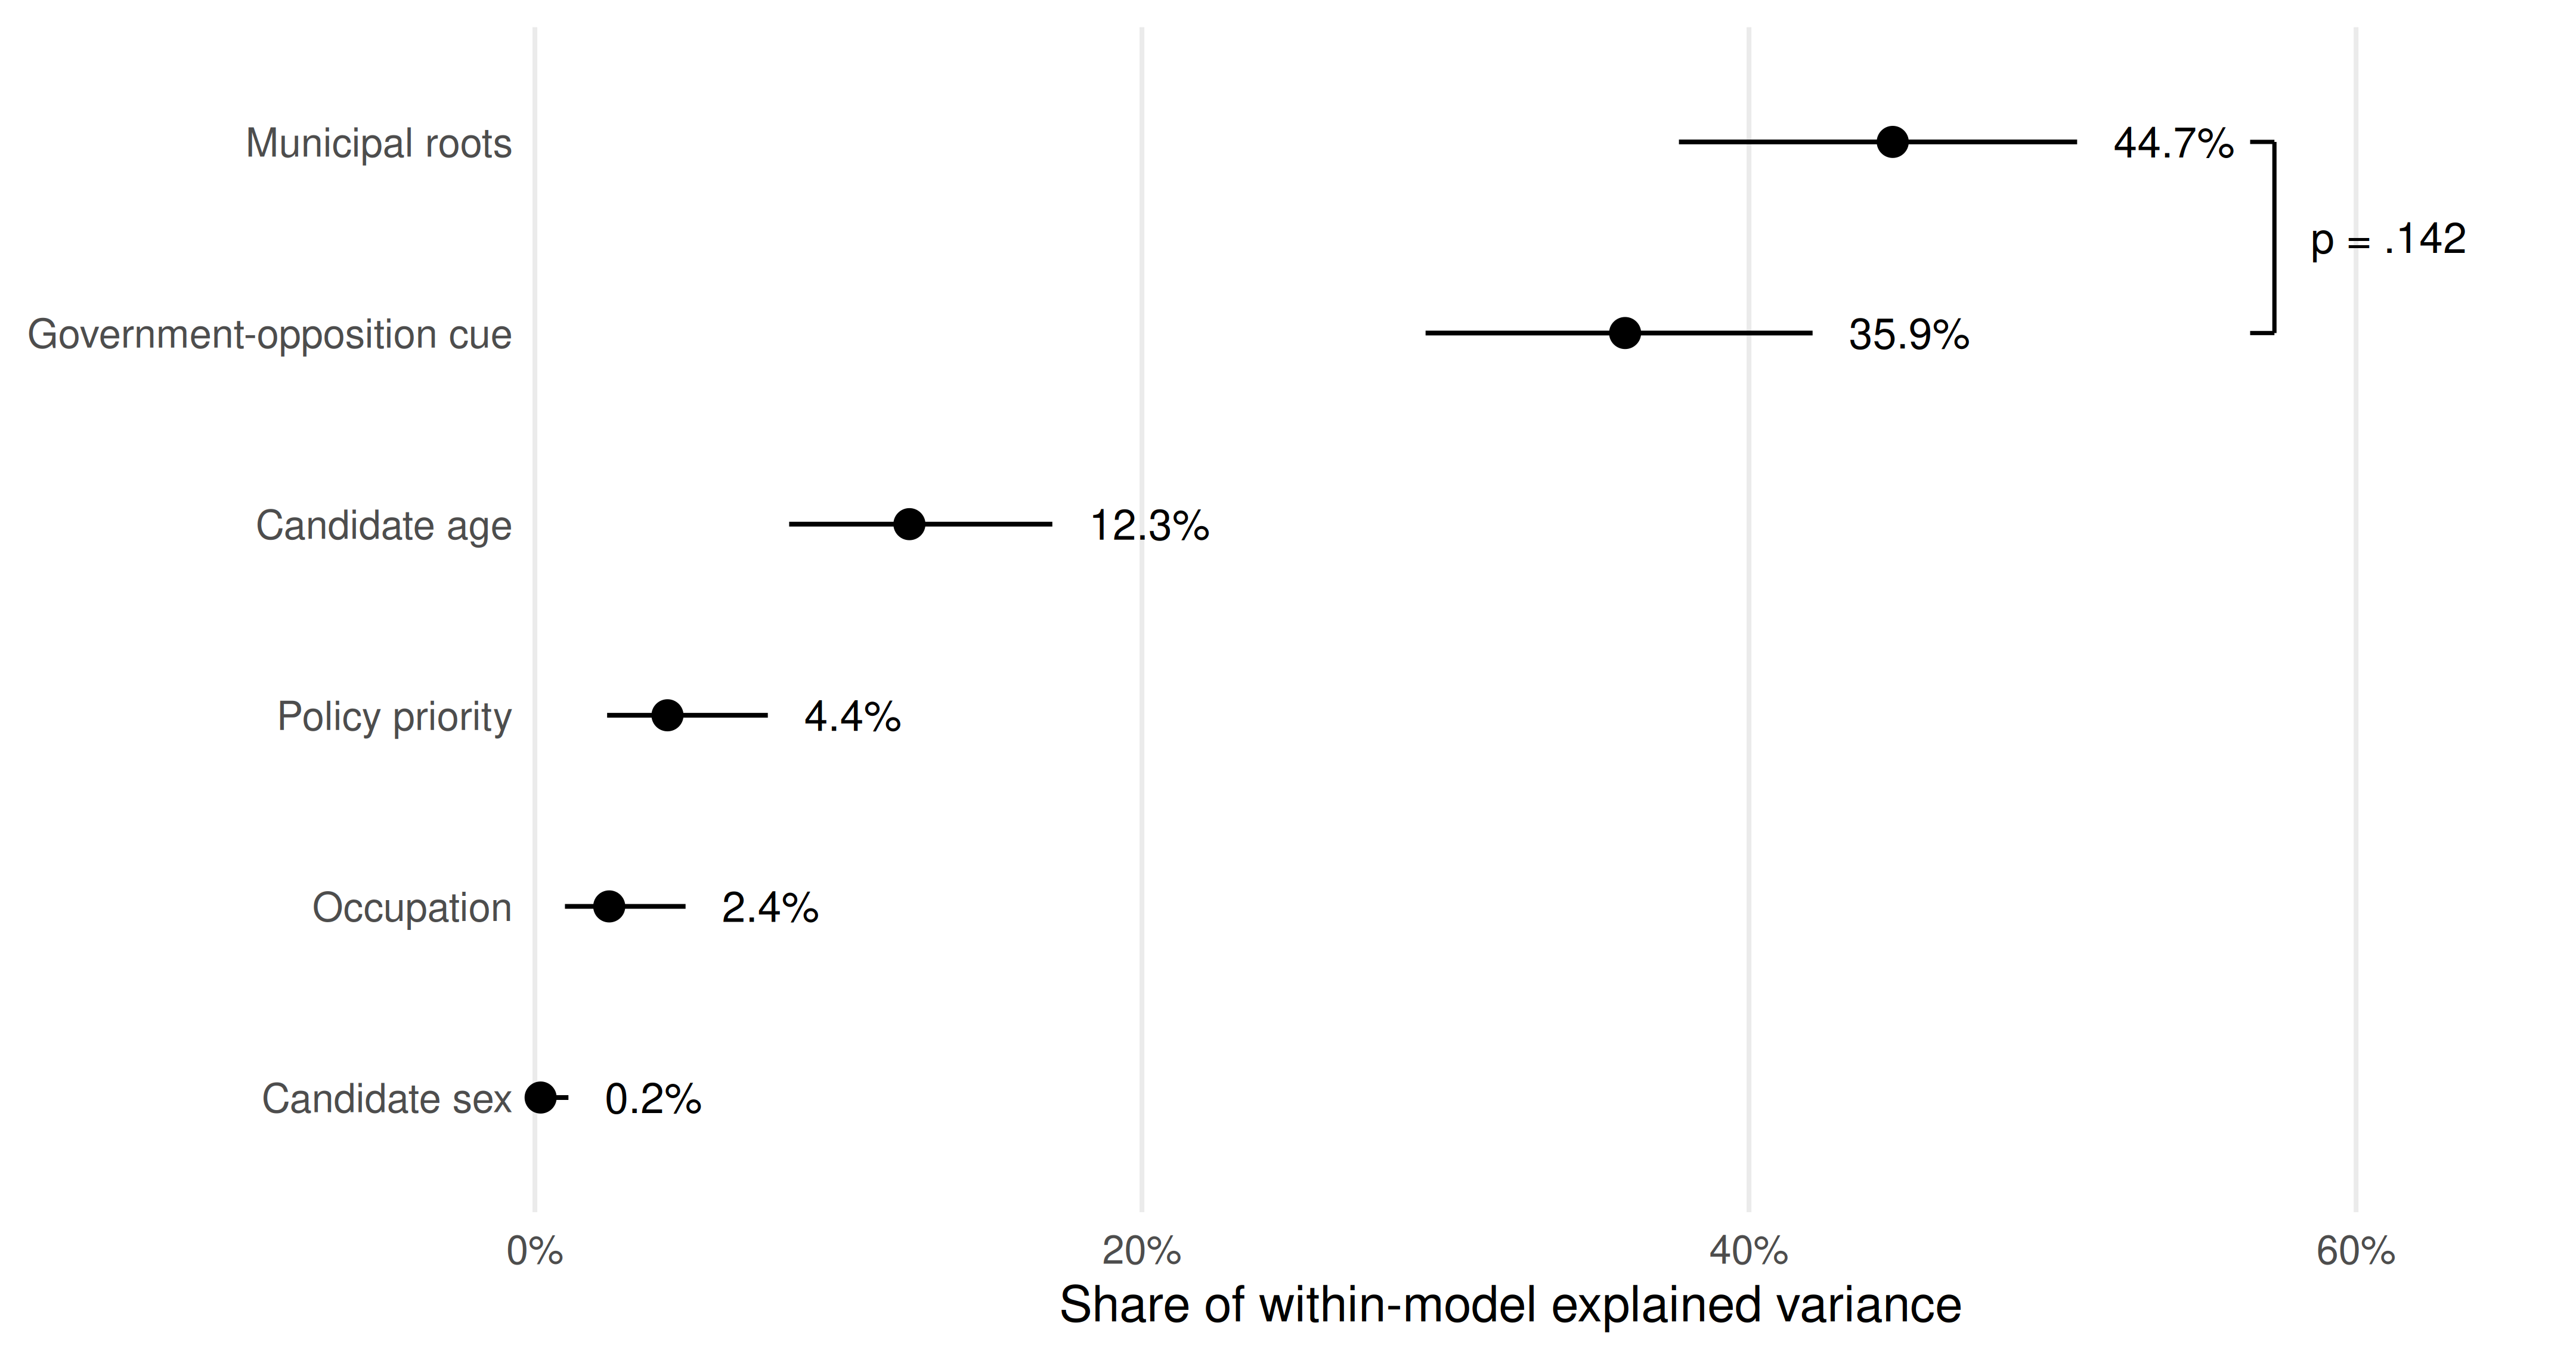
\includegraphics[width=0.8\linewidth,height=\textheight,keepaspectratio,alt={Horizontal point-and-interval plot of six candidate attributes\textquotesingle{} shares of within-model explained variance. Municipal roots have the largest point share at 44.7\%; a bracket comparing it with the 35.9\% government-opposition share reports p equals .142.}]{figs/paper_dominance.png}

}

\caption{\label{fig-dominance}\criticmarkupadd{General dominance weights
for candidate attributes. Points are normalized shares of within-model
explained variance, and bars are percentile 95\% confidence intervals
from 4,999 respondent-clustered bootstrap replicates. The bracket
reports the unadjusted two-sided centered-bootstrap p-value for the
municipal-roots minus government-cue contrast. Within-model R-squared is
0.062, and office is absorbed by respondent fixed effects.}}

\end{figure}%

\subsection{Local roots are not confined to local
offices}\label{local-roots-are-not-confined-to-local-offices}

Office-specific MMs in Figure~\ref{fig-office} show the
municipal-connection gradient in every condition. Relative to the
\criticmarkuprm{outsider-with-local-knowledge
statement,}\criticmarkupadd{outsider profile, residence for a few years
increases} the \criticmarkuprm{few-years-resident statement
increases}\criticmarkupadd{probability of} selection by 13.4 points for
MPs (95\% CI: 10.3 to 16.5), 14.0 for mayors (95\% CI: 10.8 to 17.1),
and 12.8 for councillors (95\% CI: 9.6 to 16.1).
\criticmarkuprm{Relative to the same outsider statement, the
lifelong-resident statement}\criticmarkupadd{Lifelong residence}
increases \criticmarkuprm{selection}\criticmarkupadd{it} by 19.0 points
for MPs (95\% CI: 15.9 to 22.2), 17.2 for mayors (95\% CI: 14.1 to
20.4), and 19.5 for councillors (95\% CI: 16.2 to 22.9).

The point estimates do not follow \criticmarkuprm{the predicted
office}\criticmarkupadd{a councillor--mayor--MP} ordering. The omnibus
interaction is not detected, \(F(4,2185)=0.661\), \(p=.619\). None of
the nine pairwise office comparisons within the three
municipal-connection levels is statistically distinguishable from zero
(unadjusted \(p=.141\) to \(.946\); all Holm-adjusted \(p=1.000\)).
These tests do not prove equality, but they provide no evidence that the
\criticmarkuprm{place-based cue is strongest for councillor
profiles.}\criticmarkupadd{local-roots bonus differs across the three
prompts.}

\begin{figure}

\centering{


\includegraphics[width=1\linewidth,height=\textheight,keepaspectratio,alt={Point estimates and confidence intervals for the three municipal-roots levels, shown separately for MP, mayor, and councillor profiles.}]{figs/paper_municip_by_office.png}

}

\caption{\label{fig-office}Marginal means for municipal roots by office}

\end{figure}%

\emph{Note.} MMs from an unweighted linear probability model interacting
municipal roots with office; 95\% robust, respondent-clustered
confidence intervals. The vertical line marks 0.50. Numerical
comparisons in the text are differences in MMs within office.

\subsection{Local roots and political alignment}\label{sec-main-finding}

Figure~\ref{fig-heterogeneity} compares
\criticmarkuprm{place-based}\criticmarkupadd{local-root} and
\criticmarkuprm{government-alignment
cues}\criticmarkupadd{political-alignment contrasts} among clearly pro-
and anti-government profiles and respondents. The top panel displays
marginal means across municipal-connection levels for aligned and
non-aligned pairs. The lower-left panel shows resident--outsider
differences within each alignment group; the lower-right panel shows
aligned--non-aligned differences within each municipal-connection level.

\criticmarkuprm{The municipal-statement contrasts are
positive}\criticmarkupadd{Local roots increase the probability of
selection} in both alignment groups. Relative to the
\criticmarkuprm{outsider-with-local-knowledge statement, the
few-years-resident statement}\criticmarkupadd{outsider profile,
residence for a few years} increases selection
\criticmarkupadd{probability }by 10.3 points among non-aligned pairs
(95\% CI: 7.1 to 13.4) and 13.2 points among aligned pairs (95\% CI: 9.5
to 16.9). \criticmarkuprm{Relative to the same outsider statement, the
lifelong-resident statement}\criticmarkupadd{Lifelong residence}
increases \criticmarkuprm{selection}\criticmarkupadd{it} by 14.2 points
among non-aligned pairs (95\% CI: 10.9 to 17.4) and 19.5 points among
aligned pairs (95\% CI: 16.0 to 23.0). The difference-in-differences is
2.9 points for \criticmarkuprm{the few-years-resident
statement}\criticmarkupadd{residence of a few years} (95\% CI: \(-1.9\)
to 7.8, \(p=.230\)) and 5.3 points for \criticmarkuprm{the
lifelong-resident statement}\criticmarkupadd{lifelong residence} (95\%
CI: 0.7 to 9.9, \(p=.024\); Holm-adjusted \(p=.047\)).
\criticmarkuprm{The}\criticmarkupadd{Only the lifelong-residence}
interaction is \criticmarkuprm{therefore
concentrated}\criticmarkupadd{detected} in the
\criticmarkuprm{lifelong-resident-statement
contrast.}\criticmarkupadd{primary specification.}

\criticmarkuprm{Government alignment
has}\criticmarkupadd{Political-alignment contrasts are} larger
\criticmarkuprm{point estimates.}\criticmarkupadd{in magnitude.} Aligned
profiles gain 27.9 points among outsiders (95\% CI: 24.5 to 31.3), 30.8
among residents of a few years (95\% CI: 27.3 to 34.4), and 33.2 among
lifelong residents (95\% CI: 29.8 to \criticmarkuprm{36.6).Figure
3}\criticmarkupadd{36.6). Figure~\ref{fig-heterogeneity}} highlights one
additional cross-profile contrast from the same model. An aligned
\criticmarkuprm{profile with the outsider-with-local-knowledge
statement}\criticmarkupadd{outsider} has an MM of 49.4\%, compared with
35.6\% for a non-aligned \criticmarkuprm{profile with the
lifelong-resident statement:}\criticmarkupadd{lifelong resident:} a
13.7-point \criticmarkuprm{cross-profile }difference (95\% CI: 10.0 to
\criticmarkuprm{17.5).}\criticmarkupadd{17.5). This gap indicates that
strong local roots do not offset political misalignment in this design.}

The interaction evidence \criticmarkuprm{is suggestive rather than
decisive.}\criticmarkupadd{remains exploratory.} The lifelong-residence
interaction \criticmarkuprm{remains}\criticmarkupadd{is} about 4.9--5.1
points under both \criticmarkuprm{weights}\criticmarkupadd{weighting
schemes} but does not retain Holm-adjusted significance; it is 3.5--4.8
points under alternative \criticmarkuprm{attitude
cutoffs.}\criticmarkupadd{cutoff points defining political alignment.}
The signed-advantage outcome supports a larger lifelong-residence bonus
among aligned pairs (0.90 scale points, 95\% CI: 0.26 to 1.53;
Holm-adjusted \(p=.012\)). The stable \criticmarkuprm{conclusion is
that}\criticmarkupadd{findings are positive local-root contrasts in}
both \criticmarkuprm{cues matter}\criticmarkupadd{groups} and
\criticmarkuprm{the alignment contrast is
larger;}\criticmarkupadd{larger political-alignment contrasts;} stronger
local benefits among aligned pairs require replication. Candidate
profiles contain no party label, so these estimates concern congruence
on the government--opposition cue, not a generic party effect.

\begin{figure}

\centering{


\includegraphics[width=1\linewidth,height=\textheight,keepaspectratio,alt={Three-panel black-and-white plot. The top panel compares municipal-connection marginal means for aligned and non-aligned pairs. The lower-left panel shows resident-minus-outsider differences within alignment groups. The lower-right panel shows aligned-minus-non-aligned differences within municipal-connection levels. In the top panel, thin dotted vertical guides through two reference points are joined by a horizontal line labelled 13.7 percentage points.}]{figs/paper_cue_heterogeneity.png}

}

\caption{\label{fig-heterogeneity}Municipal roots and
government--opposition alignment among clearly positioned cases}

\end{figure}%

\emph{Note.} MMs and differences in MMs from an unweighted linear
probability model with municipal-roots-by-alignment interactions,
\criticmarkuprm{a}\criticmarkupadd{an indicator for pro- versus
anti-government} respondent \criticmarkuprm{attitude-group
control,}\criticmarkupadd{attitudes,} and robust, respondent-clustered
95\% confidence intervals (\(1{,}635\) respondents; \(8{,}712\)
profiles). Aligned means pro/pro or anti/anti candidate--respondent
combinations. Non-aligned means pro/anti or anti/pro combinations.
Neutral candidate profiles and respondents scoring 4--6 are outside this
comparison. The MM panel uses a 0.50 reference line; difference panels
use zero. Open triangles and filled circles distinguish non-aligned and
aligned pairs; open circles, crosses, and filled squares distinguish
outsider, few-years-resident, and lifelong-resident statements. The
bracket highlights the additional 13.7-point cross-profile contrast
described in the text. All seven within-dimension pairwise differences
displayed in the lower panels are significant at \(\alpha=.05\): both
resident--outsider contrasts within aligned and non-aligned pairs, and
aligned--non-aligned contrasts at all three municipal-root levels
(Table~\ref{tbl-figure3-pairwise}).

\section{Discussion}\label{discussion}

The \criticmarkuprm{results support one
argument:}\criticmarkupadd{findings follow the three comparisons.
Respondents distinguish graded municipal connections; the gradient
appears in all three office prompts; and} local roots
\criticmarkuprm{matter, but they operate within rather than
outside}\criticmarkupadd{increase support among both aligned and
non-aligned pairs. Political mismatch nevertheless produces larger
probability differences, while} the \criticmarkuprm{national political
divide. The few-years-resident statement increases selection by 13.4
points relative to the outsider-with-local-knowledge statement. The
lifelong-resident statement increases selection by 18.6 points relative
to the outsider-with-local-knowledge statement. The alignment comparison
and office split locate these complete statement contrasts within the
national divide and across
offices.}\criticmarkupadd{local-roots-by-alignment interaction remains
exploratory.}

\criticmarkuprm{The 13--19-point}\criticmarkupadd{Residence for a few
years raises the probability of selection by 13.4 points relative to the
outsider profile, and lifelong residence raises it by 18.6 points. These
experimental} contrasts \criticmarkuprm{show that respondents
distinguish lifelong residents, newer residents, and outsiders even when
national political position and other candidate traits }are
\criticmarkuprm{visible. The same gradient appears for MP, mayoral, and
councillor profiles, so the local advantage is not confined to
specifically local offices. Related studies find local-root advantages
for party leaders (Put 2021), Senate candidates (Hunt 2022), and state
legislators (Hunt and Rouse 2023), while local-election research
emphasizes that their magnitude varies across candidates and settings
(Czapiewski and Woźniak 2021; Zissel 2026).
The}\criticmarkupadd{compatible with} Polish electoral-return
\criticmarkuprm{literature documents}\criticmarkupadd{evidence of} local
vote and turnout advantages (Górecki et al. 2022), \criticmarkuprm{which
can also reflect}\criticmarkupadd{while separating the presented profile
statements from} campaign contact, information diffusion, and
\criticmarkuprm{mobilization.}\criticmarkupadd{mobilization. Municipal
roots also have the largest point share in the pooled dominance
analysis, although their 8.8-point lead over the government cue is
uncertain.}

\criticmarkuprm{One explanation}\criticmarkupadd{The same gradient
appears} for \criticmarkupadd{MP, mayoral, and councillor profiles. The
omnibus and pairwise tests detect no office differences, but }the
\criticmarkuprm{office pattern is that
respondents}\criticmarkupadd{intervals do not establish equal effects.
Respondents may} use municipal connection as a general candidate-quality
cue rather than recalibrating it to \criticmarkuprm{the functional
demands of }each office. \criticmarkuprm{The identical attribute wording
and fit-for-office task may have encouraged that cross-office
interpretation. The null interaction does not imply complete
nationalization: the municipal statements produced positive contrasts in
every office, and the uncertainty is too wide to establish equal
effects. }Replication with treatments tailored to \criticmarkuprm{each
office's}\criticmarkupadd{the} territorial scale \criticmarkupadd{of
each office }would distinguish a general heuristic from office-specific
evaluations.

\criticmarkuprm{National political congruence can outweigh even strong
local roots. Aligned profiles gain}\criticmarkupadd{Political alignment
changes the probability of selection by} 28--33 \criticmarkuprm{points
over non-aligned profiles.}\criticmarkupadd{points.} An aligned
\criticmarkuprm{profile with the outsider-with-local-knowledge
statement}\criticmarkupadd{outsider} is 13.7 points more likely to be
selected than a non-aligned \criticmarkuprm{profile with the
lifelong-resident statement. Municipal
embeddedness}\criticmarkupadd{lifelong resident. Strong local roots}
therefore \criticmarkuprm{remains consequential without displacing the
national divide.}\criticmarkupadd{do not offset political mismatch.} US
experimental evidence likewise finds that local-root rewards can cross
party lines (Hunt and Fontana 2025), \criticmarkuprm{while German
local-executive evidence shows that nomination background conditions
spatial voting (Zissel 2026). Neither}\criticmarkupadd{but the present}
study \criticmarkuprm{estimates}\criticmarkupadd{directly compares local
roots with respondent-specific political alignment. The larger alignment
contrasts and} the \criticmarkuprm{government-alignment contrast used
here.}\criticmarkupadd{pooled dominance ranking answer different
questions: the former compare conditional MMs, whereas the latter
summarizes each randomized attribute's contribution across the full
sample.}

\criticmarkuprm{Municipal-statement}\criticmarkupadd{Local-root}
contrasts remain positive among both aligned and non-aligned pairs. The
5.3-point primary interaction
\criticmarkuprm{weakens}\criticmarkupadd{changes} under alternative
\criticmarkuprm{attitude}\criticmarkupadd{alignment} cutoffs and does
not retain adjusted significance under either weighting scheme. The
\criticmarkuprm{evidence therefore establishes coexistence,
not}\criticmarkupadd{stable result is coexistence; whether aligned
candidates receive} a \criticmarkuprm{stable interaction between the
cues. Place matters alongside national alignment (Munis 2021), but it
does not erase the principal partisan division in this
experiment.}\criticmarkupadd{larger local-roots bonus remains an
exploratory finding that requires replication.}

\criticmarkuprm{Three limits qualify these findings. }The
\criticmarkuprm{conjoint measures}\criticmarkupadd{design makes three
trade-offs. First, randomized profile information provides control over
candidate cues at the cost of behavioral realism: the outcome is} stated
\criticmarkuprm{profile evaluations,}\criticmarkupadd{suitability for
office,} not \criticmarkuprm{electoral behavior; prior behavioral
validation of paired conjoint effects (Hainmueller et al. 2015) does not
establish equivalence in Polish elections. The}\criticmarkupadd{an
actual vote (Hainmueller et al. 2015). Second, the} online quota sample
\criticmarkupadd{made the large split-ballot experiment feasible but }is
not a probability \criticmarkuprm{sample, and}\criticmarkupadd{sample;}
similar weighted estimates cannot eliminate selection concerns.
\criticmarkuprm{Finally,}\criticmarkupadd{Third, holding a profile
distribution fixed permits clear contrasts, but} the estimates
\criticmarkuprm{average over this experiment's profile distribution and
}may change with the prevalence or combination of candidate traits ({de
la Cuesta et al.} 2022). The
\criticmarkuprm{design}\criticmarkupadd{outsider statement adds a
realistic defense of parachute candidacy---declared local
knowledge---but therefore does not isolate residence alone. The
experiment} also cannot identify psychological mediators, canvassing,
home-area mobilization, acquaintance, or network
\criticmarkuprm{effects. Experimental and observational studies
distinguish local service, community embeddedness, ballot information,
and place identity}\criticmarkupadd{effects} (Campbell et al. 2019;
Harfst et al. 2023; Velimsky et al. 2024; Schulte-Cloos and Bauer 2023;
Nyholt 2024; Ornstein et al. 2025)\criticmarkuprm{, but the present
complete-statement contrasts do not separate those
explanations.}\criticmarkupadd{. Within these limits, randomization
identifies contrasts among the complete statements presented to this
sample.}

\section{Conclusion}\label{conclusion}

Polish respondents distinguish graded municipal
\criticmarkuprm{connections. The few-years-resident statement
increases}\criticmarkupadd{connections: residence for a few years raises
the probability of} selection by 13.4 points relative to the
\criticmarkuprm{outsider-with-local-knowledge statement. The
lifelong-resident statement increases
selection}\criticmarkupadd{outsider profile, and lifelong residence
raises it} by 18.6 \criticmarkuprm{points relative to the
outsider-with-local-knowledge statement. These statement contrasts
appear}\criticmarkupadd{points. The gradient appears} in all three
office prompts without
\criticmarkuprm{detectable}\criticmarkupadd{detected} office
differences. \criticmarkuprm{Yet they operate within the national
political divide. Among clearly positioned cases,}\criticmarkupadd{Local
roots also increase support among both} aligned \criticmarkuprm{profiles
gain}\criticmarkupadd{and non-aligned pairs. Political alignment,
however, changes selection by} 27.9--33.2 \criticmarkuprm{points.
An}\criticmarkupadd{points, and an} aligned \criticmarkuprm{profile with
the outsider-with-local-knowledge statement}\criticmarkupadd{outsider}
outperforms a non-aligned \criticmarkuprm{profile with the
lifelong-resident statement.}\criticmarkupadd{lifelong resident.} The
\criticmarkuprm{local and national}\criticmarkupadd{interaction between
these} cues \criticmarkuprm{coexist, while their interaction varies
across alternative weights and attitude cutoffs. The contribution is
relational: municipal embeddedness matters}\criticmarkupadd{remains
exploratory. Local roots therefore matter} across offices
\criticmarkuprm{without insulating candidate evaluation from
national}\criticmarkupadd{and} political
\criticmarkuprm{conflict.}\criticmarkupadd{alignments, but they do not
offset political mismatch.}

\section*{Data availability}\label{data-availability}
\addcontentsline{toc}{section}{Data availability}

The accompanying \texttt{reproduction/} directory contains the
redistributable source datasets, R analysis code, \texttt{targets}
workflow, and generated numerical results. Its pipeline regenerates the
figures used by this Quarto manuscript.

\section*{Funding}\label{funding}
\addcontentsline{toc}{section}{Funding}

The survey was conducted as part of the project ``Political
Representation of Women in Local Governments,'' funded by the National
Science Centre, Poland (grant 2021/43/B/HS5/01059).

\protect\phantomsection\label{appendix-count}
\section*{Appendix}\label{appendix}
\addcontentsline{toc}{section}{Appendix}

\subsection*{Sampling, fieldwork, and weights}\label{sec-sampling}
\addcontentsline{toc}{subsection}{Sampling, fieldwork, and weights}

Wave 1 was fielded online between 28 March and 7 April 2024. Ariadna
invited 9,534 panel members; 2,935 entered the survey, 521 did not
complete it, and 207 were removed by quality-control criteria, leaving
2,207 respondents. Quotas covered sex, five age categories, five
municipality-size categories, two education categories, and 16
voivodeships. The split-ballot assignment yielded 778 MP, 742 mayor, and
687 councillor respondents.

The released data contain two post-stratification weights. The
census-margin post-stratification weight adjusts the quota dimensions to
2021 census margins and ranges from 0.536 to 1.760 in wave 1. The census
and reported 2023-vote post-stratification weight additionally adjusts
reported turnout and party vote in the 2023 parliamentary election and
ranges from 0.229 to 3.004. The unweighted model is primary because the
experimental attributes are randomized. Table~\ref{tbl-robustness} shows
that both weighted specifications yield the same substantive
municipal-roots and government-cue pattern.

\subsection*{Split-ballot and profile randomization}\label{sec-balance}
\addcontentsline{toc}{subsection}{Split-ballot and profile
randomization}

The split-ballot groups are balanced on sex, age group, education,
municipality size, and voivodeship. Omnibus chi-square tests yield
\(p=.291\) to \(.941\) (all Holm-adjusted \(p=1.000\)), and Cramer's
\(V\) ranges from .007 to .085.

Table~\ref{tbl-balance} reports randomized attribute-level shares within
each office condition. The maximum minus minimum office share is at most
.019 across all levels, consistent with the common randomization scheme.

\begin{longtable}[]{@{}
  >{\raggedright\arraybackslash}p{(\linewidth - 10\tabcolsep) * \real{0.1667}}
  >{\raggedright\arraybackslash}p{(\linewidth - 10\tabcolsep) * \real{0.1667}}
  >{\raggedleft\arraybackslash}p{(\linewidth - 10\tabcolsep) * \real{0.1667}}
  >{\raggedleft\arraybackslash}p{(\linewidth - 10\tabcolsep) * \real{0.1667}}
  >{\raggedleft\arraybackslash}p{(\linewidth - 10\tabcolsep) * \real{0.1667}}
  >{\raggedleft\arraybackslash}p{(\linewidth - 10\tabcolsep) * \real{0.1667}}@{}}
\caption{Randomized attribute-level shares by office
condition}\label{tbl-balance}\tabularnewline
\toprule\noalign{}
\begin{minipage}[b]{\linewidth}\raggedright
Attribute
\end{minipage} & \begin{minipage}[b]{\linewidth}\raggedright
Level
\end{minipage} & \begin{minipage}[b]{\linewidth}\raggedleft
MP
\end{minipage} & \begin{minipage}[b]{\linewidth}\raggedleft
Mayor
\end{minipage} & \begin{minipage}[b]{\linewidth}\raggedleft
Councillor
\end{minipage} & \begin{minipage}[b]{\linewidth}\raggedleft
Max-min
\end{minipage} \\
\midrule\noalign{}
\endfirsthead
\toprule\noalign{}
\begin{minipage}[b]{\linewidth}\raggedright
Attribute
\end{minipage} & \begin{minipage}[b]{\linewidth}\raggedright
Level
\end{minipage} & \begin{minipage}[b]{\linewidth}\raggedleft
MP
\end{minipage} & \begin{minipage}[b]{\linewidth}\raggedleft
Mayor
\end{minipage} & \begin{minipage}[b]{\linewidth}\raggedleft
Councillor
\end{minipage} & \begin{minipage}[b]{\linewidth}\raggedleft
Max-min
\end{minipage} \\
\midrule\noalign{}
\endhead
\bottomrule\noalign{}
\endlastfoot
Candidate age & 31 & 0.248 & 0.247 & 0.251 & 0.004 \\
Candidate age & 43 & 0.259 & 0.257 & 0.248 & 0.011 \\
Candidate age & 55 & 0.244 & 0.256 & 0.246 & 0.012 \\
Candidate age & 67 & 0.249 & 0.241 & 0.255 & 0.015 \\
Candidate sex & Male & 0.494 & 0.511 & 0.492 & 0.019 \\
Candidate sex & Female & 0.506 & 0.489 & 0.508 & 0.019 \\
Occupation & Lawyer & 0.258 & 0.252 & 0.252 & 0.006 \\
Occupation & Engineer & 0.252 & 0.241 & 0.252 & 0.011 \\
Occupation & History teacher & 0.246 & 0.244 & 0.237 & 0.009 \\
Occupation & Entrepreneur & 0.245 & 0.264 & 0.259 & 0.019 \\
Government-opposition cue & Neutral & 0.334 & 0.342 & 0.334 & 0.008 \\
Government-opposition cue & Pro-government & 0.341 & 0.333 & 0.340 &
0.008 \\
Government-opposition cue & Anti-government & 0.325 & 0.325 & 0.326 &
0.001 \\
Municipal roots & Lives elsewhere; knows local issues & 0.328 & 0.337 &
0.328 & 0.009 \\
Municipal roots & Lives locally for a few years & 0.335 & 0.328 & 0.331
& 0.007 \\
Municipal roots & Lives locally since birth & 0.337 & 0.335 & 0.341 &
0.006 \\
Policy priority & Support business & 0.195 & 0.201 & 0.205 & 0.009 \\
Policy priority & Improve roads & 0.197 & 0.199 & 0.201 & 0.004 \\
Policy priority & Support families & 0.210 & 0.203 & 0.194 & 0.016 \\
Policy priority & Support older residents & 0.199 & 0.196 & 0.199 &
0.003 \\
Policy priority & Protect the environment & 0.200 & 0.201 & 0.202 &
0.003 \\
\end{longtable}

\subsection*{Task wording and coding}\label{sec-wording}
\addcontentsline{toc}{subsection}{Task wording and coding}

Respondents selected the profile better suited for the assigned office
and then rated its advantage over the alternative.
Table~\ref{tbl-task-wording} reports the Polish questionnaire wording
and a direct English translation. The respondent moderator asks: ``What
is your attitude toward the government of Donald Tusk and the coalition
currently governing Poland?'' Its scale runs from 0 (opponent) to 10
(supporter).

\begin{longtable}[]{@{}
  >{\raggedright\arraybackslash}p{(\linewidth - 4\tabcolsep) * \real{0.1800}}
  >{\raggedright\arraybackslash}p{(\linewidth - 4\tabcolsep) * \real{0.4100}}
  >{\raggedright\arraybackslash}p{(\linewidth - 4\tabcolsep) * \real{0.4100}}@{}}
\caption{Questionnaire wording and English
translation}\label{tbl-task-wording}\tabularnewline
\toprule\noalign{}
\begin{minipage}[b]{\linewidth}\raggedright
Item
\end{minipage} & \begin{minipage}[b]{\linewidth}\raggedright
Polish wording
\end{minipage} & \begin{minipage}[b]{\linewidth}\raggedright
English translation
\end{minipage} \\
\midrule\noalign{}
\endfirsthead
\toprule\noalign{}
\begin{minipage}[b]{\linewidth}\raggedright
Item
\end{minipage} & \begin{minipage}[b]{\linewidth}\raggedright
Polish wording
\end{minipage} & \begin{minipage}[b]{\linewidth}\raggedright
English translation
\end{minipage} \\
\midrule\noalign{}
\endhead
\bottomrule\noalign{}
\endlastfoot
Introduction & Za chwilę zobaczysz na ekranie kilka par {[}kandydatów na
posłów / kandydatów na radnych gminy (miasta) / kandydatów na wójta
(burmistrza){]}. & In a moment, you will see several pairs of
{[}candidates for members of parliament / candidates for municipal
(city) councillors / candidates for commune head (mayor){]}. \\
Pair-review instruction & Obejrzyj dokładnie każdą parę i wskaż, która z
dwóch osób według Ciebie lepiej nadaje się na {[}posła lub posłankę /
radnego lub radną / wójta (burmistrza){]}. & Examine each pair carefully
and indicate which of the two people, in your opinion, is better suited
to be {[}a member of parliament / a municipal councillor / a commune
head (mayor){]}. \\
Forced-choice instruction & Nawet jeśli nie jesteś do końca
przekonany/-a lub nie podobają Ci się obie przedstawione opcje, wskaż
tę, która jest choć trochę lepsza niż druga. & Even if you are not
entirely certain or dislike both options presented, indicate the one
that is at least slightly better than the other. \\
Occupation (8) & Zawód (8): inżynier / inżynierka / prawnik / prawniczka
/ nauczyciel historii / nauczycielka historii / właściciel małej firmy /
właścicielka małej firmy & Occupation (8): engineer (male/female
wording) / lawyer (male/female wording) / history teacher (male/female
wording) / small-business owner (male/female wording) \\
Age (4) & Wiek (4): 31 lat / 43 lata / 55 lat / 67 lat & Age (4): 31 /
43 / 55 / 67 years \\
Attitude toward the current government (3) & Stosunek do obecnego rządu
(3): wspiera rząd D. Tuska i partie koalicji rządzącej / jest w opozycji
do rządu D. Tuska i partii koalicji rządzącej / zajmuje neutralne
stanowisko wobec rządu D. Tuska i partii koalicji rządzącej & Attitude
toward the current government (3): supports Donald Tusk's government and
the governing coalition parties / is in opposition to Donald Tusk's
government and the governing coalition parties / takes a neutral
position toward Donald Tusk's government and the governing coalition
parties \\
Residence (3) & Zamieszkanie (3): mieszka w mieście/gminie od urodzenia
/ mieszka w mieście/gminie od kilku lat / mieszka w innym
mieście/gminie, ale deklaruje że zna problemy tej okolicy & Residence
(3): has lived in the town/municipality since birth / has lived in the
town/municipality for a few years / lives in another town/municipality
but states that they know the problems of the local area \\
Important policy proposal (5) & Ważny postulat (5): więcej wsparcia dla
rodzin / więcej wsparcia dla seniorów / więcej wsparcia dla
przedsiębiorców / więcej troski o środowisko i klimat / więcej troski o
jakość dróg & Important policy proposal (5): more support for families /
more support for older residents / more support for entrepreneurs / more
attention to the environment and climate / more attention to road
quality \\
Q48 \texttt{conjoint\ competence} & Która osoba nadaje się lepiej na ten
urząd? & Which person is better suited to this office? \\
Q48 response format & {[}binarny{]} & {[}binary{]} \\
Q49 \texttt{conjointvote} & Oceń w skali od 0 do 10 jak duża jest
przewaga wybranej przez Ciebie osoby nad tą drugą? & On a scale from 0
to 10, rate how large the advantage of the person you selected is over
the other person. \\
Q49 response scale & {[}skala od 0 -- minimalna przewaga do 10 --
ogromna przewaga, bez trudno powiedzieć{]} & {[}scale from 0---minimal
advantage---to 10---enormous advantage; no ``difficult to say''
option{]} \\
\end{longtable}

\begin{longtable}[]{@{}
  >{\raggedright\arraybackslash}p{(\linewidth - 2\tabcolsep) * \real{0.5000}}
  >{\raggedright\arraybackslash}p{(\linewidth - 2\tabcolsep) * \real{0.5000}}@{}}
\caption{Outcome coding}\label{tbl-outcomes}\tabularnewline
\toprule\noalign{}
\begin{minipage}[b]{\linewidth}\raggedright
Measure
\end{minipage} & \begin{minipage}[b]{\linewidth}\raggedright
Analysis coding
\end{minipage} \\
\midrule\noalign{}
\endfirsthead
\toprule\noalign{}
\begin{minipage}[b]{\linewidth}\raggedright
Measure
\end{minipage} & \begin{minipage}[b]{\linewidth}\raggedright
Analysis coding
\end{minipage} \\
\midrule\noalign{}
\endhead
\bottomrule\noalign{}
\endlastfoot
Forced choice (Q48) & Selected profile = 1; other profile = 0 \\
Advantage (Q49) & Selected profile = 0 to 10; other profile = 0 to
-10 \\
\end{longtable}

The advantage ratings indicate clear choices in most tasks: 83.1\% are
at or above the scale midpoint and 48.6\% fall between 7 and 10.

\begin{longtable}[]{@{}rrr@{}}
\caption{Distribution of the selected profile's advantage
rating}\label{tbl-advantage-distribution}\tabularnewline
\toprule\noalign{}
Advantage rating & Number of tasks & Percent \\
\midrule\noalign{}
\endfirsthead
\toprule\noalign{}
Advantage rating & Number of tasks & Percent \\
\midrule\noalign{}
\endhead
\bottomrule\noalign{}
\endlastfoot
0 & 201 & 2.3 \\
1 & 222 & 2.5 \\
2 & 316 & 3.6 \\
3 & 357 & 4.0 \\
4 & 400 & 4.5 \\
5 & 1503 & 17.0 \\
6 & 1542 & 17.5 \\
7 & 1750 & 19.8 \\
8 & 1314 & 14.9 \\
9 & 571 & 6.5 \\
10 & 652 & 7.4 \\
\end{longtable}

The alignment coding is:

\begin{itemize}
\tightlist
\item
  aligned: pro-government candidate with a respondent scoring 7--10, or
  anti-government candidate with a respondent scoring 0--3;
\item
  non-aligned: pro-government candidate with a respondent scoring 0--3,
  or anti-government candidate with a respondent scoring 7--10.
\end{itemize}

Neutral candidate profiles and respondents scoring 4--6 are excluded
from the primary alignment comparison. Alternative respondent cutoffs
are reported in the
\hyperref[sec-alignment-sensitivity]{alignment-sensitivity appendix}.

\subsection*{Model specifications}\label{sec-models}
\addcontentsline{toc}{subsection}{Model specifications}

For profile \(j\) in task \(t\) evaluated by respondent \(i\), the
pooled model underlying Figure~\ref{fig-main-effects} is

\[
Y_{ijt}=\alpha+\sum_{a}\sum_{l\neq 0}\beta_{al}D_{ijtal}+\boldsymbol{\delta}^{\mathsf T}\mathbf{O}_{i}+\varepsilon_{ijt},
\]

where \(D_{ijtal}\) indexes non-reference level \(l\) of randomized
attribute \(a\), and \(\mathbf{O}_{i}\) contains office-condition
indicators. All confidence intervals and tests use
heteroskedasticity-robust standard errors clustered by respondent.
Figure~\ref{fig-office} replaces the additive municipal-roots and office
terms with their full interaction:

\[
Y_{ijt}=\alpha+\boldsymbol{\beta}^{\mathsf T}\mathbf{X}_{ijt}+\boldsymbol{\gamma}^{\mathsf T}(\mathbf{M}_{ijt}\times\mathbf{O}_{i})+\varepsilon_{ijt}.
\]

Figure~\ref{fig-heterogeneity} analogously interacts municipal roots
\(\mathbf{M}_{ijt}\) with the binary alignment measure
\(\mathbf{A}_{ijt}\) and
\criticmarkuprm{controls}\criticmarkupadd{includes an indicator} for the
respondent's pro- or anti-government attitude group \(\mathbf{R}_{i}\):

\[
Y_{ijt}=\alpha+\boldsymbol{\beta}^{\mathsf T}\mathbf{X}_{ijt}+\boldsymbol{\theta}^{\mathsf T}(\mathbf{M}_{ijt}\times\mathbf{A}_{ijt})+\boldsymbol{\rho}^{\mathsf T}\mathbf{R}_{i}+\boldsymbol{\delta}^{\mathsf T}\mathbf{O}_{i}+\varepsilon_{ijt}.
\]

In the second and third equations, \(\mathbf{X}_{ijt}\) contains the
remaining randomized attributes. In the alignment model, the randomized
government cue enters through \(\mathbf{A}_{ijt}\) rather than as a
separate additive term. Reported conditional results are predictions
averaged over the analyzed profile distribution and their linear
contrasts, not the raw interaction coefficients.

\subsection*{Pairwise contrasts displayed in Figure
3}\label{pairwise-contrasts-displayed-in-figure-3}
\addcontentsline{toc}{subsection}{Pairwise contrasts displayed in Figure
3}

Table~\ref{tbl-figure3-pairwise} reports the seven pairwise contrasts
displayed in Figure~\ref{fig-heterogeneity}. Holm adjustment treats the
seven displayed comparisons as one family.

\begin{longtable}[]{@{}
  >{\raggedright\arraybackslash}p{(\linewidth - 12\tabcolsep) * \real{0.1429}}
  >{\raggedright\arraybackslash}p{(\linewidth - 12\tabcolsep) * \real{0.1429}}
  >{\raggedright\arraybackslash}p{(\linewidth - 12\tabcolsep) * \real{0.1429}}
  >{\raggedleft\arraybackslash}p{(\linewidth - 12\tabcolsep) * \real{0.1429}}
  >{\raggedright\arraybackslash}p{(\linewidth - 12\tabcolsep) * \real{0.1429}}
  >{\raggedleft\arraybackslash}p{(\linewidth - 12\tabcolsep) * \real{0.1429}}
  >{\raggedleft\arraybackslash}p{(\linewidth - 12\tabcolsep) * \real{0.1429}}@{}}
\caption{Pairwise contrasts displayed in Figure
3}\label{tbl-figure3-pairwise}\tabularnewline
\toprule\noalign{}
\begin{minipage}[b]{\linewidth}\raggedright
Panel comparison
\end{minipage} & \begin{minipage}[b]{\linewidth}\raggedright
Condition
\end{minipage} & \begin{minipage}[b]{\linewidth}\raggedright
Contrast
\end{minipage} & \begin{minipage}[b]{\linewidth}\raggedleft
Difference (points)
\end{minipage} & \begin{minipage}[b]{\linewidth}\raggedright
95\% CI
\end{minipage} & \begin{minipage}[b]{\linewidth}\raggedleft
Raw \(p\)
\end{minipage} & \begin{minipage}[b]{\linewidth}\raggedleft
Holm \(p\)
\end{minipage} \\
\midrule\noalign{}
\endfirsthead
\toprule\noalign{}
\begin{minipage}[b]{\linewidth}\raggedright
Panel comparison
\end{minipage} & \begin{minipage}[b]{\linewidth}\raggedright
Condition
\end{minipage} & \begin{minipage}[b]{\linewidth}\raggedright
Contrast
\end{minipage} & \begin{minipage}[b]{\linewidth}\raggedleft
Difference (points)
\end{minipage} & \begin{minipage}[b]{\linewidth}\raggedright
95\% CI
\end{minipage} & \begin{minipage}[b]{\linewidth}\raggedleft
Raw \(p\)
\end{minipage} & \begin{minipage}[b]{\linewidth}\raggedleft
Holm \(p\)
\end{minipage} \\
\midrule\noalign{}
\endhead
\bottomrule\noalign{}
\endlastfoot
Municipal statement & Non-aligned & Few-years resident minus outsider
with local knowledge & 10.3 & 7.1, 13.4 & \(1.96 \times 10^{-10}\) &
\(1.96 \times 10^{-10}\) \\
Municipal statement & Non-aligned & Lifelong resident minus outsider
with local knowledge & 14.2 & 10.9, 17.4 & \(2.43 \times 10^{-17}\) &
\(7.28 \times 10^{-17}\) \\
Municipal statement & Aligned & Few-years resident minus outsider with
local knowledge & 13.2 & 9.5, 16.9 & \(3.58 \times 10^{-12}\) &
\(7.16 \times 10^{-12}\) \\
Municipal statement & Aligned & Lifelong resident minus outsider with
local knowledge & 19.5 & 16.0, 23.0 & \(6.61 \times 10^{-27}\) &
\(2.65 \times 10^{-26}\) \\
Political alignment & Outsider with local knowledge & Aligned minus
non-aligned & 27.9 & 24.5, 31.3 & \(2.80 \times 10^{-55}\) &
\(1.40 \times 10^{-54}\) \\
Political alignment & Few-years resident & Aligned minus non-aligned &
30.8 & 27.3, 34.4 & \(3.55 \times 10^{-60}\) &
\(2.13 \times 10^{-59}\) \\
Political alignment & Lifelong resident & Aligned minus non-aligned &
33.2 & 29.8, 36.6 & \(1.23 \times 10^{-73}\) &
\(8.59 \times 10^{-73}\) \\
\end{longtable}

\emph{Note.} Differences are percentage points from the unweighted
alignment model, with heteroskedasticity-robust standard errors
clustered by respondent. Confidence intervals are 95\%. Raw and
Holm-adjusted p-values come from the same seven model-based linear
contrasts plotted in Figure~\ref{fig-heterogeneity}.

\subsection*{Alignment-coding
sensitivity}\label{sec-alignment-sensitivity}
\addcontentsline{toc}{subsection}{Alignment-coding sensitivity}

The primary 0--3 and 7--10 \criticmarkuprm{respondent
cutoffs}\criticmarkupadd{endpoints} are operational choices rather than
natural breaks in the \criticmarkupadd{attitude }scale.
Table~\ref{tbl-alignment-sensitivity} repeats the aligned--non-aligned
contrasts using narrower (0--2 versus 8--10) and broader (0--4 versus
6--10) \criticmarkuprm{definitions.}\criticmarkupadd{definitions of
political alignment.} The estimates remain positive at every
municipal-connection level and retain the same ordering relative to the
residence contrasts. Their exact magnitude declines as the respondent
groups broaden.

\begin{longtable}[]{@{}
  >{\raggedright\arraybackslash}p{(\linewidth - 10\tabcolsep) * \real{0.1667}}
  >{\raggedright\arraybackslash}p{(\linewidth - 10\tabcolsep) * \real{0.1667}}
  >{\raggedleft\arraybackslash}p{(\linewidth - 10\tabcolsep) * \real{0.1667}}
  >{\raggedleft\arraybackslash}p{(\linewidth - 10\tabcolsep) * \real{0.1667}}
  >{\raggedleft\arraybackslash}p{(\linewidth - 10\tabcolsep) * \real{0.1667}}
  >{\raggedright\arraybackslash}p{(\linewidth - 10\tabcolsep) * \real{0.1667}}@{}}
\caption{Sensitivity of aligned--non-aligned contrasts to alternative
definitions of political
alignment}\label{tbl-alignment-sensitivity}\tabularnewline
\toprule\noalign{}
\begin{minipage}[b]{\linewidth}\raggedright
Coding
\end{minipage} & \begin{minipage}[b]{\linewidth}\raggedright
Municipal-roots level
\end{minipage} & \begin{minipage}[b]{\linewidth}\raggedleft
Respondents
\end{minipage} & \begin{minipage}[b]{\linewidth}\raggedleft
Profiles
\end{minipage} & \begin{minipage}[b]{\linewidth}\raggedleft
Aligned minus non-aligned
\end{minipage} & \begin{minipage}[b]{\linewidth}\raggedright
95\% CI
\end{minipage} \\
\midrule\noalign{}
\endfirsthead
\toprule\noalign{}
\begin{minipage}[b]{\linewidth}\raggedright
Coding
\end{minipage} & \begin{minipage}[b]{\linewidth}\raggedright
Municipal-roots level
\end{minipage} & \begin{minipage}[b]{\linewidth}\raggedleft
Respondents
\end{minipage} & \begin{minipage}[b]{\linewidth}\raggedleft
Profiles
\end{minipage} & \begin{minipage}[b]{\linewidth}\raggedleft
Aligned minus non-aligned
\end{minipage} & \begin{minipage}[b]{\linewidth}\raggedright
95\% CI
\end{minipage} \\
\midrule\noalign{}
\endhead
\bottomrule\noalign{}
\endlastfoot
Narrow: 0-2 vs 8-10 & Lives elsewhere; knows local issues & 1381 & 7366
& 0.300 & 0.263, 0.337 \\
Narrow: 0-2 vs 8-10 & Lives locally for a few years & 1381 & 7366 &
0.324 & 0.286, 0.363 \\
Narrow: 0-2 vs 8-10 & Lives locally since birth & 1381 & 7366 & 0.335 &
0.298, 0.372 \\
Primary: 0-3 vs 7-10 & Lives elsewhere; knows local issues & 1635 & 8712
& 0.279 & 0.245, 0.313 \\
Primary: 0-3 vs 7-10 & Lives locally for a few years & 1635 & 8712 &
0.308 & 0.273, 0.344 \\
Primary: 0-3 vs 7-10 & Lives locally since birth & 1635 & 8712 & 0.332 &
0.298, 0.366 \\
Broad: 0-4 vs 6-10 & Lives elsewhere; knows local issues & 1841 & 9776 &
0.259 & 0.227, 0.291 \\
Broad: 0-4 vs 6-10 & Lives locally for a few years & 1841 & 9776 & 0.299
& 0.265, 0.333 \\
Broad: 0-4 vs 6-10 & Lives locally since birth & 1841 & 9776 & 0.307 &
0.274, 0.340 \\
\end{longtable}

\emph{Note.} Entries are differences in marginal means from the
alignment model, with robust, respondent-clustered 95\% confidence
intervals. Respondents between the indicated endpoint groups and neutral
candidate profiles are excluded. The respondent and profile counts are
constant across the three municipal-connection rows within each coding.

\subsubsection*{Interaction robustness}\label{interaction-robustness}
\addcontentsline{toc}{subsubsection}{Interaction robustness}

Table~\ref{tbl-interaction-robustness} reports whether the local bonus
differs between aligned and non-aligned pairs. Holm adjustment covers
the two municipal contrasts within each specification.

\begin{longtable}[]{@{}
  >{\raggedright\arraybackslash}p{(\linewidth - 10\tabcolsep) * \real{0.1667}}
  >{\raggedright\arraybackslash}p{(\linewidth - 10\tabcolsep) * \real{0.1667}}
  >{\raggedright\arraybackslash}p{(\linewidth - 10\tabcolsep) * \real{0.1667}}
  >{\raggedleft\arraybackslash}p{(\linewidth - 10\tabcolsep) * \real{0.1667}}
  >{\raggedright\arraybackslash}p{(\linewidth - 10\tabcolsep) * \real{0.1667}}
  >{\raggedleft\arraybackslash}p{(\linewidth - 10\tabcolsep) * \real{0.1667}}@{}}
\caption{Robustness of municipal-connection-by-alignment
interactions}\label{tbl-interaction-robustness}\tabularnewline
\toprule\noalign{}
\begin{minipage}[b]{\linewidth}\raggedright
Coding/outcome
\end{minipage} & \begin{minipage}[b]{\linewidth}\raggedright
Weight
\end{minipage} & \begin{minipage}[b]{\linewidth}\raggedright
Municipal contrast
\end{minipage} & \begin{minipage}[b]{\linewidth}\raggedleft
Difference-in-differences
\end{minipage} & \begin{minipage}[b]{\linewidth}\raggedright
95\% CI
\end{minipage} & \begin{minipage}[b]{\linewidth}\raggedleft
Holm \(p\)
\end{minipage} \\
\midrule\noalign{}
\endfirsthead
\toprule\noalign{}
\begin{minipage}[b]{\linewidth}\raggedright
Coding/outcome
\end{minipage} & \begin{minipage}[b]{\linewidth}\raggedright
Weight
\end{minipage} & \begin{minipage}[b]{\linewidth}\raggedright
Municipal contrast
\end{minipage} & \begin{minipage}[b]{\linewidth}\raggedleft
Difference-in-differences
\end{minipage} & \begin{minipage}[b]{\linewidth}\raggedright
95\% CI
\end{minipage} & \begin{minipage}[b]{\linewidth}\raggedleft
Holm \(p\)
\end{minipage} \\
\midrule\noalign{}
\endhead
\bottomrule\noalign{}
\endlastfoot
Narrow forced choice & None & Few years local & .024 & -.028, .077 &
.363 \\
Narrow forced choice & None & Local since birth & .035 & -.015, .085 &
.334 \\
Primary forced choice & None & Few years local & .029 & -.019, .078 &
.230 \\
Primary forced choice & None & Local since birth & .053 & .007, .099 &
.047 \\
Primary forced choice & Census margins & Few years local & .024 & -.025,
.074 & .337 \\
Primary forced choice & Census margins & Local since birth & .051 &
.004, .098 & .066 \\
Primary forced choice & Census + 2023 vote & Few years local & .030 &
-.025, .084 & .286 \\
Primary forced choice & Census + 2023 vote & Local since birth & .049 &
-.002, .100 & .116 \\
Primary signed advantage & None & Few years local & .245 & -.410, .899 &
.463 \\
Primary signed advantage & None & Local since birth & .896 & .259, 1.534
& .012 \\
Broad forced choice & None & Few years local & .040 & -.006, .085 &
.089 \\
Broad forced choice & None & Local since birth & .048 & .004, .092 &
.069 \\
\end{longtable}

\emph{Note.} Forced-choice estimates are probability differences;
signed-advantage estimates are points on the \(-10\) to \(10\) scale.
Positive values indicate a larger local bonus among aligned pairs.

\subsection*{Tabular model estimates}\label{sec-estimates}
\addcontentsline{toc}{subsection}{Tabular model estimates}

Table~\ref{tbl-model-estimates} reports the coefficients from the
unweighted pooled linear probability model used for the AMCE panel in
Figure~\ref{fig-main-effects}. Office coefficients are close to zero by
construction because exactly one profile is selected in each pair and
office is assigned at respondent level; the office-specific quantities
of interest in Figure~\ref{fig-office} come from interactions with
municipal roots.

\begin{longtable}[]{@{}
  >{\raggedright\arraybackslash}p{(\linewidth - 6\tabcolsep) * \real{0.2500}}
  >{\raggedleft\arraybackslash}p{(\linewidth - 6\tabcolsep) * \real{0.2500}}
  >{\raggedleft\arraybackslash}p{(\linewidth - 6\tabcolsep) * \real{0.2500}}
  >{\raggedright\arraybackslash}p{(\linewidth - 6\tabcolsep) * \real{0.2500}}@{}}
\caption{Pooled unweighted linear probability
model}\label{tbl-model-estimates}\tabularnewline
\toprule\noalign{}
\begin{minipage}[b]{\linewidth}\raggedright
Term
\end{minipage} & \begin{minipage}[b]{\linewidth}\raggedleft
Estimate
\end{minipage} & \begin{minipage}[b]{\linewidth}\raggedleft
Std. error
\end{minipage} & \begin{minipage}[b]{\linewidth}\raggedright
95\% CI
\end{minipage} \\
\midrule\noalign{}
\endfirsthead
\toprule\noalign{}
\begin{minipage}[b]{\linewidth}\raggedright
Term
\end{minipage} & \begin{minipage}[b]{\linewidth}\raggedleft
Estimate
\end{minipage} & \begin{minipage}[b]{\linewidth}\raggedleft
Std. error
\end{minipage} & \begin{minipage}[b]{\linewidth}\raggedright
95\% CI
\end{minipage} \\
\midrule\noalign{}
\endhead
\bottomrule\noalign{}
\endlastfoot
Intercept & 0.539 & 0.015 & 0.510, 0.568 \\
Age: 43 vs 31 & -0.004 & 0.011 & -0.025, 0.016 \\
Age: 55 vs 31 & -0.035 & 0.011 & -0.055, -0.014 \\
Age: 67 vs 31 & -0.103 & 0.011 & -0.124, -0.081 \\
Female vs male & 0.010 & 0.007 & -0.005, 0.024 \\
Engineer vs lawyer & 0.013 & 0.011 & -0.008, 0.034 \\
History teacher vs lawyer & -0.037 & 0.011 & -0.058, -0.016 \\
Entrepreneur vs lawyer & -0.002 & 0.010 & -0.022, 0.019 \\
Pro-government vs neutral & -0.109 & 0.010 & -0.129, -0.090 \\
Anti-government vs neutral & -0.172 & 0.010 & -0.191, -0.153 \\
Few years local vs outsider & 0.134 & 0.009 & 0.116, 0.152 \\
Local since birth vs outsider & 0.186 & 0.009 & 0.167, 0.204 \\
Improve roads vs support business & -0.019 & 0.012 & -0.042, 0.004 \\
Support families vs support business & 0.034 & 0.012 & 0.010, 0.058 \\
Support older residents vs support business & -0.019 & 0.012 & -0.043,
0.004 \\
Environment vs support business & -0.037 & 0.012 & -0.060, -0.013 \\
Mayor vs MP prompt & 0.000 & 0.002 & -0.004, 0.005 \\
Councillor vs MP prompt & 0.001 & 0.002 & -0.003, 0.005 \\
\end{longtable}

\subsection*{Weighting and alternative-outcome
robustness}\label{sec-robustness}
\addcontentsline{toc}{subsection}{Weighting and alternative-outcome
robustness}

Table~\ref{tbl-robustness} compares the four focal AMCEs across the
unweighted model, the census-margin post-stratified model, and the
census plus reported 2023-vote post-stratified model. It also reports
the unweighted signed-advantage model. Weighting changes some pooled
government coefficients because those cues interact with respondent
orientations, but it does not change the direction or substantive
conclusion. Municipal-roots estimates remain positive under every
specification.

For the alternative outcome, respondents rated the selected profile's
advantage from 0 to 10. Across the 8,828 tasks, all scale points occur
in the data. The selected profile retains the non-negative value and the
unselected profile receives its negative, producing a symmetric
profile-level scale from \(-10\) to \(10\). On this scale, living
locally for a few years increases the advantage by 1.79 points and
lifelong residence by 2.48 points; pro-government and anti-government
cues reduce it by 1.43 and 2.28 points, respectively, relative to
neutrality.

\begin{longtable}[]{@{}
  >{\raggedright\arraybackslash}p{(\linewidth - 10\tabcolsep) * \real{0.1667}}
  >{\raggedright\arraybackslash}p{(\linewidth - 10\tabcolsep) * \real{0.1667}}
  >{\raggedright\arraybackslash}p{(\linewidth - 10\tabcolsep) * \real{0.1667}}
  >{\raggedright\arraybackslash}p{(\linewidth - 10\tabcolsep) * \real{0.1667}}
  >{\raggedleft\arraybackslash}p{(\linewidth - 10\tabcolsep) * \real{0.1667}}
  >{\raggedright\arraybackslash}p{(\linewidth - 10\tabcolsep) * \real{0.1667}}@{}}
\caption{Robustness of focal cue
estimates}\label{tbl-robustness}\tabularnewline
\toprule\noalign{}
\begin{minipage}[b]{\linewidth}\raggedright
Outcome
\end{minipage} & \begin{minipage}[b]{\linewidth}\raggedright
Weight
\end{minipage} & \begin{minipage}[b]{\linewidth}\raggedright
Attribute
\end{minipage} & \begin{minipage}[b]{\linewidth}\raggedright
Contrast
\end{minipage} & \begin{minipage}[b]{\linewidth}\raggedleft
Estimate
\end{minipage} & \begin{minipage}[b]{\linewidth}\raggedright
95\% CI
\end{minipage} \\
\midrule\noalign{}
\endfirsthead
\toprule\noalign{}
\begin{minipage}[b]{\linewidth}\raggedright
Outcome
\end{minipage} & \begin{minipage}[b]{\linewidth}\raggedright
Weight
\end{minipage} & \begin{minipage}[b]{\linewidth}\raggedright
Attribute
\end{minipage} & \begin{minipage}[b]{\linewidth}\raggedright
Contrast
\end{minipage} & \begin{minipage}[b]{\linewidth}\raggedleft
Estimate
\end{minipage} & \begin{minipage}[b]{\linewidth}\raggedright
95\% CI
\end{minipage} \\
\midrule\noalign{}
\endhead
\bottomrule\noalign{}
\endlastfoot
Signed advantage & None & Government-opposition cue & Anti-government vs
neutral & -2.279 & -2.538, -2.020 \\
Signed advantage & None & Government-opposition cue & Pro-government vs
neutral & -1.431 & -1.699, -1.163 \\
Signed advantage & None & Municipal roots & Few years local vs outsider
& 1.786 & 1.542, 2.030 \\
Signed advantage & None & Municipal roots & Local since birth vs
outsider & 2.480 & 2.231, 2.729 \\
Forced choice & None & Government-opposition cue & Anti-government vs
neutral & -0.172 & -0.191, -0.153 \\
Forced choice & None & Government-opposition cue & Pro-government vs
neutral & -0.109 & -0.129, -0.090 \\
Forced choice & None & Municipal roots & Few years local vs outsider &
0.134 & 0.116, 0.152 \\
Forced choice & None & Municipal roots & Local since birth vs outsider &
0.186 & 0.167, 0.204 \\
Forced choice & Census-margin post-stratification &
Government-opposition cue & Anti-government vs neutral & -0.173 &
-0.193, -0.154 \\
Forced choice & Census-margin post-stratification &
Government-opposition cue & Pro-government vs neutral & -0.114 & -0.134,
-0.094 \\
Forced choice & Census-margin post-stratification & Municipal roots &
Few years local vs outsider & 0.127 & 0.108, 0.146 \\
Forced choice & Census-margin post-stratification & Municipal roots &
Local since birth vs outsider & 0.184 & 0.165, 0.203 \\
Forced choice & Census + reported 2023-vote post-stratification &
Government-opposition cue & Anti-government vs neutral & -0.149 &
-0.170, -0.129 \\
Forced choice & Census + reported 2023-vote post-stratification &
Government-opposition cue & Pro-government vs neutral & -0.143 & -0.165,
-0.121 \\
Forced choice & Census + reported 2023-vote post-stratification &
Municipal roots & Few years local vs outsider & 0.118 & 0.098, 0.139 \\
Forced choice & Census + reported 2023-vote post-stratification &
Municipal roots & Local since birth vs outsider & 0.178 & 0.158,
0.199 \\
\end{longtable}

\emph{Note.} Forced-choice coefficients are probability differences;
advantage coefficients are points on the signed \(-10\) to \(10\)
profile scale. All models use robust, respondent-clustered standard
errors and include all randomized profile attributes plus office
indicators.

\section*{References}\label{references}
\addcontentsline{toc}{section}{References}

\protect\phantomsection\label{refs}
\begin{CSLReferences}{1}{1}
\bibitem[\citeproctext]{ref-arterpoyet2024}
Arter, David, and Corentin Poyet. 2024. {``{{`Importing'}} the Personal
Vote to Maximise the Party Vote? {{`Parachute Personalization'}} in an
Intraparty Preference Electoral System.''} \emph{Politics} 44 (4).
\url{https://doi.org/10.1177/02633957241267754}.

\bibitem[\citeproctext]{ref-arzheimer2012}
Arzheimer, Kai, and Jocelyn Evans. 2012. {``Geolocation and Voting:
Candidate-Voter Distance Effects on Party Choice in the 2010 {UK}
General Election in England.''} \emph{Political Geography} 31 (5):
301--10. \url{https://doi.org/10.1016/j.polgeo.2012.04.006}.

\bibitem[\citeproctext]{ref-azenbudescu2003}
Azen, Razia, and David V. Budescu. 2003. {``The Dominance Analysis
Approach for Comparing Predictors in Multiple Regression.''}
\emph{Psychological Methods} 8 (2): 129--48.
\url{https://doi.org/10.1037/1082-989X.8.2.129}.

\bibitem[\citeproctext]{ref-berz2022}
Berz, Jan, and Michael Jankowski. 2022. {``Local Preferences in
Candidate Selection: Evidence from a Conjoint Experiment Among Party
Leaders in Germany.''} \emph{Party Politics} 28 (6): 1136--49.
\url{https://doi.org/10.1177/13540688211041770}.

\bibitem[\citeproctext]{ref-bowler1993}
Bowler, Shaun, Todd Donovan, and Joseph Snipp. 1993. {``Local Sources of
Information and Voter Choice in State Elections: Microlevel Foundations
of the Friends-and-Neighbors Effect.''} \emph{American Politics
Quarterly} 21 (4): 473--89.
\url{https://doi.org/10.1177/1532673X9302100405}.

\bibitem[\citeproctext]{ref-budescu1993}
Budescu, David V. 1993. {``Dominance Analysis: A New Approach to the
Problem of Relative Importance of Predictors in Multiple Regression.''}
\emph{Psychological Bulletin} 114 (3): 542--51.
\url{https://doi.org/10.1037/0033-2909.114.3.542}.

\bibitem[\citeproctext]{ref-campbellcowley2014}
Campbell, Rosie, and Philip Cowley. 2014. {``What Voters Want: Reactions
to Candidate Characteristics in a Survey Experiment.''} \emph{Political
Studies} 62 (4): 745--65. \url{https://doi.org/10.1111/1467-9248.12048}.

\bibitem[\citeproctext]{ref-campbell2019}
Campbell, Rosie, Philip Cowley, Nick Vivyan, and Markus Wagner. 2019.
{``Why Friends and Neighbors? Explaining the Electoral Appeal of Local
Roots.''} \emph{The Journal of Politics} 81 (3): 937--51.
\url{https://doi.org/10.1086/703131}.

\bibitem[\citeproctext]{ref-czapiewski2021}
Czapiewski, Tomasz, and Monika Woźniak. 2021. {``Friends and Neighbours
Voting in Local Elections in Open List System: Evidence from Poland.''}
\emph{Athenaeum. Polskie Studia Politologiczne} 72: 168--87.
\url{https://doi.org/10.15804/athena.2021.72.10}.

\bibitem[\citeproctext]{ref-delacuesta2022}
{de la Cuesta, Brandon, Naoki Egami, and Kosuke Imai}. 2022.
{``Improving the External Validity of Conjoint Analysis: The Essential
Role of Profile Distribution.''} \emph{Political Analysis} 30 (1):
19--45. \url{https://doi.org/10.1017/pan.2020.40}.

\bibitem[\citeproctext]{ref-egami2019}
Egami, Naoki, and Kosuke Imai. 2019. {``Causal Interaction in Factorial
Experiments: Application to Conjoint Analysis.''} \emph{Journal of the
American Statistical Association} 114 (526): 529--40.
\url{https://doi.org/10.1080/01621459.2018.1476246}.

\bibitem[\citeproctext]{ref-evans2017}
Evans, Jocelyn, Kai Arzheimer, Rosie Campbell, and Philip Cowley. 2017.
{``Candidate Localness and Voter Choice in the 2015 General Election in
England.''} \emph{Political Geography} 59: 61--71.
\url{https://doi.org/10.1016/j.polgeo.2017.02.009}.

\bibitem[\citeproctext]{ref-DVN_LKY4WZ_2025}
Gendzwill, Adam, and Jan Kroszka. 2025. \emph{{Polish Local Election
Study 2024 - panel survey}}. Version V1. Harvard Dataverse.
\url{https://doi.org/10.7910/DVN/LKY4WZ}.

\bibitem[\citeproctext]{ref-gendzwill2012}
Gendźwiłł, Adam. 2012. {``Independent Mayors and Local Lists in Large
Polish Cities: Towards a Non-Partisan Model of Local Government?''}
\emph{Local Government Studies} 38 (4): 501--18.
\url{https://doi.org/10.1080/03003930.2011.649915}.

\bibitem[\citeproctext]{ref-gendzwillkjaer2023}
Gendźwiłł, Adam, and Ulrik Kjaer. 2023. {``The Second-Order Election
Model and the Performance of Political Parties in Municipal
Elections.''} \emph{Party Politics} 29 (6): 1178--85.
\url{https://doi.org/10.1177/13540688221117245}.

\bibitem[\citeproctext]{ref-gimpel2008}
Gimpel, James G., Kimberly A. Karnes, John McTague, and Shanna
Pearson-Merkowitz. 2008. {``Distance-Decay in the Political Geography of
Friends-and-Neighbors Voting.''} \emph{Political Geography} 27 (2):
231--52. \url{https://doi.org/10.1016/j.polgeo.2007.10.005}.

\bibitem[\citeproctext]{ref-gorecki2022}
Górecki, Maciej A., Sławomir Bartnicki, and Maciej Alimowski. 2022.
{``Local Voting at Local Elections Revisited: Friends and Neighbors
Voting at Mayoral Elections in Rural Poland.''} \emph{Political
Geography} 94: 102559.
\url{https://doi.org/10.1016/j.polgeo.2021.102559}.

\bibitem[\citeproctext]{ref-gorecki2012}
Górecki, Maciej A., and Michael Marsh. 2012. {``Not Just {`Friends and
Neighbours'}: Canvassing, Geographic Proximity and Voter Choice.''}
\emph{European Journal of Political Research} 51 (5): 563--82.
\url{https://doi.org/10.1111/j.1475-6765.2011.02008.x}.

\bibitem[\citeproctext]{ref-hainmueller2015}
Hainmueller, Jens, Dominik Hangartner, and Teppei Yamamoto. 2015.
{``Validating Vignette and Conjoint Survey Experiments Against
Real-World Behavior.''} \emph{Proceedings of the National Academy of
Sciences} 112 (8): 2395--400.
\url{https://doi.org/10.1073/pnas.1416587112}.

\bibitem[\citeproctext]{ref-hainmueller2014}
Hainmueller, Jens, Daniel J. Hopkins, and Teppei Yamamoto. 2014.
{``Causal Inference in Conjoint Analysis: Understanding Multidimensional
Choices via Stated Preference Experiments.''} \emph{Political Analysis}
22 (1): 1--30. \url{https://doi.org/10.1093/pan/mpt024}.

\bibitem[\citeproctext]{ref-harfst2023}
Harfst, Philipp, Damien Bol, André Blais, et al. 2023. {``All
(Electoral) Politics Is Local? Candidate's Regional Roots and Vote
Choice.''} \emph{Journal of Elections, Public Opinion and Parties} 34
(3): 387--408. \url{https://doi.org/10.1080/17457289.2023.2189257}.

\bibitem[\citeproctext]{ref-hunt2022}
Hunt, Charles R. 2022. {``Won't You Be My Senator? Nuanced Friends and
Neighbors Voting in {U.S.} Senate Elections, 1968--2018.''}
\emph{Electoral Studies} 80: 102540.
\url{https://doi.org/10.1016/j.electstud.2022.102540}.

\bibitem[\citeproctext]{ref-huntfontana2025}
Hunt, Charles R., and David Fontana. 2025. {``Is Some Politics Still
Local? Voter Preferences for Local Candidates.''} \emph{Political
Behavior} 47 (1): 167--89.
\url{https://doi.org/10.1007/s11109-024-09946-6}.

\bibitem[\citeproctext]{ref-huntrouse2023}
Hunt, Charles Russell, and Stella Rouse. 2023. {``Local Candidate Roots
and Electoral Advantages in {US} State Legislatures.''} \emph{State
Politics \& Policy Quarterly} 23 (2): 233--43.
\url{https://doi.org/10.1017/spq.2023.5}.

\bibitem[\citeproctext]{ref-jankowski2016}
Jankowski, Michael. 2016. {``Voting for Locals: Voters' Information
Processing Strategies in Open-List {PR} Systems.''} \emph{Electoral
Studies} 43: 72--84.
\url{https://doi.org/10.1016/j.electstud.2016.06.005}.

\bibitem[\citeproctext]{ref-key1949}
Key, V. O. 1949. \emph{Southern Politics in State and Nation}. Alfred A.
Knopf.

\bibitem[\citeproctext]{ref-lauredlawsk2006}
Lau, Richard R., and David P. Redlawsk. 2006. \emph{How Voters Decide:
Information Processing in Election Campaigns}. Cambridge University
Press. \url{https://doi.org/10.1017/CBO9780511791048}.

\bibitem[\citeproctext]{ref-leeper2020}
Leeper, Thomas J., Sara B. Hobolt, and James Tilley. 2020. {``Measuring
Subgroup Preferences in Conjoint Experiments.''} \emph{Political
Analysis} 28 (2): 207--21. \url{https://doi.org/10.1017/pan.2019.30}.

\bibitem[\citeproctext]{ref-lewisbeck1983}
Lewis-Beck, Michael S., and Tom W. Rice. 1983. {``Localism in
Presidential Elections: The Home State Advantage.''} \emph{American
Journal of Political Science} 27 (3): 548--56.
\url{https://doi.org/10.2307/2110984}.

\bibitem[\citeproctext]{ref-lupia1994}
Lupia, Arthur. 1994. {``Shortcuts Versus Encyclopedias: Information and
Voting Behavior in California Insurance Reform Elections.''}
\emph{American Political Science Review} 88 (1): 63--76.

\bibitem[\citeproctext]{ref-munis2021}
Munis, B. Kal. 2021. {``Place, Candidate Roots, and Voter Preferences in
an Age of Partisan Polarization: Observational and Experimental
Evidence.''} \emph{Political Geography} 85: 102345.
\url{https://doi.org/10.1016/j.polgeo.2021.102345}.

\bibitem[\citeproctext]{ref-munisburke2023}
Munis, B. Kal, and Richard Burke. 2023. {``Talk Local to Me: Assessing
the Heterogeneous Effects of Localistic Appeals.''} \emph{American
Politics Research} 51 (5): 655--69.
\url{https://doi.org/10.1177/1532673X231173402}.

\bibitem[\citeproctext]{ref-nyholt2024}
Nyholt, Niels. 2024. {``Why Do Voters Prefer Local Candidates? Evidence
from a Danish Conjoint Survey Experiment.''} \emph{Political Behavior}
46: 2313--32. \url{https://doi.org/10.1007/s11109-024-09919-9}.

\bibitem[\citeproctext]{ref-ornstein2025}
Ornstein, Joseph T., Amanda J. Heideman, Bryant J. Moy, and Kaylyn
Jackson Schiff. 2025. {``Hometown Advantage: Voter Preferences for
Community Embeddedness in Local Contests.''} \emph{Journal of
Experimental Political Science} 12 (3): 267--81.
\url{https://doi.org/10.1017/XPS.2024.16}.

\bibitem[\citeproctext]{ref-panagopoulosbailey2020}
Panagopoulos, Costas, and Kendall Bailey. 2020.
{``{{`Friends-and-Neighbors'}} Mobilization: A Field Experimental
Replication and Extension.''} \emph{Journal of Experimental Political
Science} 7 (1): 13--26. \url{https://doi.org/10.1017/XPS.2019.1}.

\bibitem[\citeproctext]{ref-panagopoulos2017}
Panagopoulos, Costas, Jan E. Leighley, and Brian T. Hamel. 2017. {``Are
Voters Mobilized by a {{`Friend-and-Neighbor'}} on the Ballot? Evidence
from a Field Experiment.''} \emph{Political Behavior} 39 (4): 865--82.
\url{https://doi.org/10.1007/s11109-016-9383-3}.

\bibitem[\citeproctext]{ref-popkin1991}
Popkin, Samuel L. 1991. \emph{The Reasoning Voter: Communication and
Persuasion in Presidential Campaigns}. The University of Chicago Press.

\bibitem[\citeproctext]{ref-put2021}
Put, Gert-Jan. 2021. {``Is There a Friends-and-Neighbors Effect for
Party Leaders?''} \emph{Electoral Studies} 71: 102338.
\url{https://doi.org/10.1016/j.electstud.2021.102338}.

\bibitem[\citeproctext]{ref-put2020}
{Put, Gert-Jan, Åsa von Schoultz, and Veikko Isotalo}. 2020. {``Fighting
over Friends and Neighbors: The Effect of Inter-Candidate Geographic
Distance on Intra-Party Competition.''} \emph{Political Geography} 81:
102219. \url{https://doi.org/10.1016/j.polgeo.2020.102219}.

\bibitem[\citeproctext]{ref-rice1987}
Rice, Tom W., and Alisa A. Macht. 1987. {``Friends and Neighbors Voting
in Statewide General Elections.''} \emph{American Journal of Political
Science} 31 (2): 448--52. \url{https://doi.org/10.2307/2111084}.

\bibitem[\citeproctext]{ref-schultecloos2023}
Schulte-Cloos, Julia, and Paul C. Bauer. 2023. {``Local Candidates,
Place-Based Identities, and Electoral Success.''} \emph{Political
Behavior} 45 (2): 679--98.
\url{https://doi.org/10.1007/s11109-021-09712-y}.

\bibitem[\citeproctext]{ref-schwarz2022}
Schwarz, Susanne, and Alexander Coppock. 2022. {``What Have We Learned
about Gender from Candidate Choice Experiments? A Meta-Analysis of
Sixty-Seven Factorial Survey Experiments.''} \emph{The Journal of
Politics} 84 (2): 655--68. \url{https://doi.org/10.1086/716290}.

\bibitem[\citeproctext]{ref-shugart2005}
Shugart, Matthew Søberg, Melody Ellis Valdini, and Kati Suominen. 2005.
{``Looking for Locals: Voter Information Demands and Personal
Vote-Earning Attributes of Legislators Under Proportional
Representation.''} \emph{American Journal of Political Science} 49 (2):
437--49. \url{https://doi.org/10.1111/j.0092-5853.2005.00133.x}.

\bibitem[\citeproctext]{ref-tavits2010}
Tavits, Margit. 2010. {``Effect of Local Ties on Electoral Success and
Parliamentary Behaviour: The Case of Estonia.''} \emph{Party Politics}
16 (2): 215--35. \url{https://doi.org/10.1177/1354068809341053}.

\bibitem[\citeproctext]{ref-tworzecki2019}
Tworzecki, Hubert. 2019. {``Poland: A Case of Top-down Polarization.''}
\emph{The ANNALS of the American Academy of Political and Social
Science} 681 (1): 97--119.
\url{https://doi.org/10.1177/0002716218809322}.

\bibitem[\citeproctext]{ref-velimsky2024}
Velimsky, Jan A., Sebastian Block, Martin Gross, and Dominic Nyhuis.
2024. {``Probing the Effect of Candidate Localness in Low-Information
Elections: Evidence from the German Local Level.''} \emph{Political
Studies} 72 (3): 1090--111.
\url{https://doi.org/10.1177/00323217231173505}.

\bibitem[\citeproctext]{ref-zissel2026}
Zissel, Pierre. 2026. {``Friends-and-Neighbours Voting in German Local
Elections: Who Is Affected by Geographic Proximity?''} \emph{Local
Government Studies}, 1--25.
\url{https://doi.org/10.1080/03003930.2026.2676815}.

\end{CSLReferences}




\end{document}
